\chapter{CONTROLLING OUTPUT}
% !TEX root = hazy1.tex
\label{sec:ControllingOutput}

\section{Overview}

\Cloudy\ is capable of generating lots of output although its
default output is minimal.
Commands that control the output are described here.
A Chapter in Hazy 2
describes the meaning of the output.  The output commands are split into
two broad classes: 
\begin{itemize}
\item\cdCommand{print} commands generate output in the
default output of the code, 
\item\cdCommand{save} commands generate output in separate files, typically
once per zone, or once per iteration.
\end{itemize}

\section{No buffering}

This command is described in Section~\ref{sec:no_buffering}.

\section{Normalize to ``O  3'' 5006.84 [scale factor = 100]}

The strength of an emission line in the standard output will be given
in intensity or luminosity units and as its intensity relative to a reference
line.  In the main printout each emission line has a label and wavelength,
followed by the energy radiated in the line, ending with the intensity
relative to a reference line.

Emission-line intensities are usually listed relative to the intensity
of H$\beta\ \lambda 4861$\AA, the default reference line.  By default the reference line
has an intensity of unity.  This command can change the reference line to
any of the other predicted lines and can change the relative intensity of
the reference line to another value.  The relative intensities of all lines
in the spectrum will be relative to the intensity of the line whose label
is within the double quotes and with wavelength given by the first number.
The label must be the four-character string that identifies the line in
the print out\footnote{The label was optional in versions 94 and before of the code, but
now is required due to the large number of lines, making unique wavelengths
unusual.}
and the wavelength must match the printed wavelength to
all four figures.
The wavelength units must appear if they are not
Angstroms.

The optional second number sets the relative intensity of the reference
line.
If it is equal to 100, as in this example, then all intensities will
be relative to a reference line intensity of 100.
The default is for an
intensity of unity.
The example given above will cause the relative
intensities to be expressed relative to an [O III] $\lambda$5006.84 intensity of 100.
The scale factor must be greater than zero.

The code works by finding the first line in the emission-line stack whose
wavelength and label matches the line on this command.
There is a possible
uniqueness problem since more than one line can have the same wavelength.
This is especially true for XUV or soft X-ray lines and for \htwo\ lines.

The following shows some examples of the \cdCommand{normalize} command:
\begin{verbatim}
# normalize to spectrum to Pa
normalize to "H  1" 1.875m

# normalize spectrum to the [OI] IR line on a scale where it is equal to 100
normalize to ``O  1'' 63.17m = 100
\end{verbatim}

\section{Print ages}

The code normally assumes that the system is old enough for microphysical
processes to have become time steady.  This tells the code to print all
of the timescales tracked by the code.
These are the same timescales
considered by the \cdCommand{age} command.
Normally only
the shortest timescale is printed at the end of the calculation.

If a physical process is not significant, for instance, the \htwo\ formation
timescale in a $10^6$~K gas,
the age is still computed but is set to a negative
number.
This retains the value while not including the process when the
important timescales are determined.


\section{Print arrays}

These commands are intended mainly as debugging aids.

\subsection{Print arrays ionization}

This prints the array elements that enter into solution
of the ionization balance.
By default it will print this information for
all elements.
If the keyword \cdCommand{only} appears then it will also look for the
name of an element and will only print the array
elements for that element.
\cdCommand{Print arrays ionization only element} commands are additive.
If more than one appears then only the information for the
requested elements will be printed.
This is a debugging aid.

\subsection{Print arrays levels ``species''}
\label{sec:PrintArraysLevels}

\par
This prints the matrix that enters the solver
for the level populations of a species.
Only one species per simulation may be specified.
The output consists of a header line followed by the rows
of the linear algebra system to solve.
The syntax for specifying levels is that of
\cdCommand{save species levels populations},
Section~\ref{sec:SaveSpeciesLevelPopulations}.
For instance, to obtain the rows and columns for all levels
the species name must be followed by the ``[:]'' notation,
e.g., ``C+[:]''.
A subset may be specified by entering the desired levels
in the brackets, e.g., ``C+[1:5]'' will print rows 1--5
and columns 1--5 of the matrix.


\section{Print citation}

\Cloudy\ is a research project that involves the creative efforts of many
people.  It should be cited as follows:  ``Calculations were performed with
version yy.mm.dd of \Cloudy, last described by Ferland et al. (yyyy).''
The numbers represent the release date and the citation is to a review paper.
The citation should mention the version of the code since some predictions
changes as the atomic data and treatment of physical processes improve.
Old versions of the code are never deleted from the web site so it is
possible to recover a version that produced a given result.

This command will print the current version number of the code and give
the full bibliographic citation for the review paper.

\section{Print constants}

The physical constants stored in the header file \cdFilename{physconst.h} will be
printed along with sizes of some variables.

\section{Print column densities [on; off]}

This controls whether the column densities of the various constituents
are printed.  The keywords are \cdCommand{\_ON\_} and \cdCommand{\_OFF}.  The default is to print the
column densities.

The column densities of several excited states within ground terms of
some species are printed as well.  The meaning of the labels for the excited
states column densities is given in the discussion of \cdTerm{cdColm} in Part 2 of
this document.

\section{Print coolants, zone 135}

This prints the coolants for the specified zone.
If no zone number or
0 appears on the line then the coolants for \emph{all} zones will be printed.
The total cooling and the fractional contribution of the strongest coolants
are printed.  For each coolant a label gives an indication of the
spectroscopic origin of the coolant and the following integer gives its
wavelength, with a 0 to indicate a continuum.  The last number of the group
is the fraction of the total cooling carried by that agent.

\section{Print continuum indices}

The file created by the \cdCommand{save continuum} command
identifies a line that occurs within each continuum bin.
This can be used
to understand what lines contribute to the predicted spectrum.
The line
label is for the first line that was entered in a particular cell.
It is
not the strongest line and there may be many lines contributing to a
particular cell.
This command will print the line energy (Rydberg),
continuum array index, and the line's spectroscopic notation, for every
line that is included in the calculation.
The lines will be printed in
the order in which they are entered into the continuum.
The printout can
then be sorted by energy or array index to discover all lines that occur
within a particular cell.
This is a debugging aid.

There are two optional numbers which give the lower and upper limit to
the energy range (Rydbergs) to be printed.
All lines are printed if these
numbers do not appear then.

\section{Print departure coefficients [He-like] [element]}

LTE departure coefficients for levels within an element along the H-like
or He-like isoelectronic sequences will be printed.
The \cdCommand{print populations}
command controls printing individual level populations.

If the keywords \cdCommand{H-like} or \cdCommand{He-like} appear,
then an element on the hydrogen-like or helium-like
isoelectronic sequences will be printed.
Otherwise all iso-sequences of the chosen element will be printed.
The code will search for the name of
an element, and if it finds one, will print only that element.
If no
elements are recognized then departure coefficients for all elements of the chosen
iso-sequence are printed.
If neither elements and iso-sequences are given or recognized, departure coefficients for
all elements and all iso-sequences will be printed.

\section{Print critical densities [He-like] [element]}

Critical densities for angular momentum changing ($l$-changing) collisions for
each element will be printed from $n=3$ for the H-like of He-like iso-sequences. 

If the keywords \cdCommand{H-like} or \cdCommand{He-like} appear,
then an element on the hydrogen-like or helium-like
isoelectronic sequences will be printed.
Otherwise all iso-sequences of the chosen element will be printed.
The code will search for the name of
an element, and if it finds one, will print only that element.
If no
elements are recognized then departure coefficients for all elements of the chosen
iso-sequence are printed.
If neither elements and iso-sequences are given or recognized, critical
densities for all elements and all iso-sequences will be printed.

\section{Print errors}

The code will always identify problems by either printing comments during
the calculation or warnings after the calculation is complete.
This says
to also print these warnings to \cdFilename{stderr}.
On many systems this output can
be redirected to the screen.
The \cdCommand{no buffering} command describes how to handle
\cdFilename{stderr} output.

\section{Print fixits}

Print a list of issues within the code which have been noted using the
\verb|fixit()| macro in the source, and where this code has been used
in the current run.

\section{Print every 1000 [5 37 93]}

This will be replaced with the \cdCommand{print zone} command.

\section{Print heating}

The relative heating due to each stage of ionization or physical process
is printed.
This is the fraction of the total heating due to this particular
stage of ionization and is printed directly below the relative abundance
of that stage.

\section{Print populations  [H-like carbon, to level 45]}

Level populations are normally not printed for the atoms and ions of
the H-like or He-like isoelectronic sequences.
This will print them.
If
no numbers appear on the line then the first 15 levels will be printed.
Enter the highest level to print on the line as an integer if more are
desired.

If the keywords \cdCommand{H-like} or \cdCommand{He-like} appear,
then an element on the hydrogen-like or helium-like
isoelectronic sequences will be printed.
Otherwise all iso-sequences of the chosen element will be printed.
The code will search for the name of
an element, and if it finds one, will print only that element.
If no
elements are recognized then departure coefficients for all elements of the chosen
iso-sequence are printed.
If neither elements and iso-sequences are given or recognized, populations for
all elements and all iso-sequences will be printed.

The departure coefficients are printed with the \cdCommand{print departure
coefficients} command.

\section{Print last}

Normally results for every iteration are printed as they are computed.
This command says to print only results for the last iteration.

\section{Print line options}

A large block of emission-line intensities is printed after the
calculation is complete.\footnote{In versions 87 and before, the code printed some relative line
intensities for each zone.  An extra line could be added with the \cdCommand{print
line} command.  This command, and that printout, no longer exists.  Use the
\cdCommand{save line intensities} command instead.} This controls details of that printout.

Some options change the layout of this information.
These include options
to print a single column, to sort the lines by wavelength or intensity,
or to print only the strongest lines, or those within a certain wavelength
range.

Other options indicate line-formation processes.
A great deal of
information about line formation and beaming is stored within the code but
not normally printed to save space.
The section of Part 2 of this document
\cdSectionTitle{The Emission Lines} gives more information.

Some spectra have so many lines that several different transitions may
appear to have the same wavelength.
This occurs to some extent for most
\htwo, \feii, and He-like spectra.
The \cdCommand{print line precision} command allows you to change the number of digits in
the printed line wavelength.
It may be necessary to increase the wavelength
precision if the default line wavelengths are ambiguous and more than one
transition appears with the same wavelength.

\subsection{Print line all}

All of the contributions to line formation, including collisions, pumping,
and heating, will be printed.

\subsection{Print line cell xx}

More than one line can occur within a continuum cell in the output
produced by the \cdCommand{save continuum} command.
This command will print the label for every line that falls into a particular
continuum cell.
The number of the cell, with the lowest energy cell being 1,
must appear.

\subsection{Print line collisions}

Collisions are often the dominant contributor to an optically thick
resonance line.
This adds an entry with the label \cdCommand{Coll}
followed by the wavelength and the collisional contribution.

\subsection{Print line column [linear]}

The main block of emission lines is normally printed with four lines
across the page.
This command says to print lines as a single column to
make it easier to enter into a spreadsheet.
The keyword \cdCommand{linear} will cause
the intensities to be printed as the linear flux in exponential format rather than as the log.

\subsection{Print line cumulative}
\label{sec:CommandPrintLineCumulative}

In a time-dependent simulation the main block of emission
lines give the emission for the current time step.
This command says to also print the time-integrated line emission,
referred to as the cumulative emission.
This ``spectrum'' is the total energy emitted in the lines,
with units $\ergpscm$.

\subsection{Print line faint -2 [\_off]}

\Cloudy\ will normally print the intensities of all emission lines with
intensities greater than $10^{-3}$ of the reference line,
which is usually H$\beta$.
This changes the limit to the relative intensity of the weakest line to
be printed.
The argument is either the log (if $\le 0$) or the linear (if
positive) intensity of the weakest line to print, relative to the reference line.
The \cdCommand{\_log} option will force interpretation as a log.
The reference
line is usually H$\beta$,
and can be changed with the \cdCommand{normalize} command.
In the case shown here, only lines with intensities
greater than 1\% of H$\beta$ will be printed.

If no numbers are entered, but the keyword \cdCommand{\_off} appears then all lines
are printed, even those with zero intensity.

\subsection{Print line flux at Earth}
\label{sec:line:flux:earth}

If the distance to an object is set with the
\cdCommand{distance} command and line luminosities are predicted
then this command says to print the observed
flux at the Earth rather than the line luminosity.
The units are ergs cm$^{-2}\mathrm{s}^{-1}$.
(No correction for interstellar extinction is included, of course).
Both the keywords \cdCommand{flux} and \cdCommand{Earth} must appear.
This command can be
combined with the \cdCommand{aperture}
command to simulate observing only part of
a spatially-resolved object.

\subsection{Print line heat}

Fluorescent excitation is included as a line formation process.
If a line is radiatively excited but then collisionally deexcited
it will heat rather than cool the gas.
This option prints the heating due to line
collisional de-excitation.
The entry will have the label \cdCommand{Heat} followed
by the wavelength.

\subsection{Print line H2 electronic}

By default only ro-vibrational lines within the ground electronic state
of \htwo\ are included in the emission-line printout when the
large \htwo\ molecule
is included with the \cdCommand{database H2} command.
This command
tells the code to also print electronic transitions.

\subsection{Print line inward}

Optically-thick emission lines are not emitted isotropically.
The
``inward'' fraction of the line is the part that is emitted from the
illuminated face of the cloud into the direction towards the source of
ionizing radiation.
This will generally be greater than 50\% of the total
intensity if the line is optically thick.
This command prints this inward
fraction with the label ``Inwd'' followed by the wavelength.

The optical depth scale must be fully converged for the inward
intensity to be predicted.
Use the \cdCommand{iterate to convergence} to do this.

\subsection{Print line iso collapsed off}
\label{sec:CommandPrintLineIsoCollapsed}

The model atoms for the iso-electronic sequences have both resolved and
collapsed levels.
Predictions from the collapsed levels can be unreliable 
below the critical density for $L$-mixing at a given $n$.
This command will disable printing predictions from the collapsed
levels.

\subsection{Print line [intrinsic, emergent] off}

By default the main line block is printed in the main output.
This command will inhibit the reporting of line intensities in
the main output, leading to significantly smaller output files.
If the keywords \cdCommand{intrinsic} or \cdCommand{emergent}
appear, then only the intrinsic or the emergent, respectively,
block of lines will be inhibited.

\subsection{Print line optical depths [\_off, faint]}
\label{sec:PrintLineOptDep}

Mean line optical depths are not printed by default\footnote{Line center optical
depths were printed through version C10.  Mean line optical depths
are now reported.  Line center optical depths are 
$\sqrt{ \pi}$  times smaller than mean optical depths.}.
The option tells the
code to print them at the end of the iteration.
For each emission line, the information printed is the species
label followed by the wavelength, the total line optical depth,
which includes contributions from overlapping emission lines,
and finally the line optical depth due to that emission line
only.

There are two optional
keywords.

If \cdCommand{\_off} appears then line mean optical depths will not be printed.  This is
useful if turned on in a previous iteration and no longer needed.

The keyword \cdCommand{faint} sets the smallest line mean optical depth to print.
The
default smallest mean line optical depth to print is 0.1.
The log of the limit
must be given.
Optical depths for all lines that mase are printed.

\subsection{Print line precision [4, 5, or 6]}

This changes the number of decimal places for line wavelengths in the final pages of
output.
Emission-line wavelengths are normally printed with six digits,
as in ``4861.36A''.
This command can change the number of digits to 4, 5 or 6.
The lines are printed in four columns when four digits are chosen.
With five or six digits the lines will no longer fit across the page so
the number of columns is automatically reduced to three.


\subsection{Print line pump}

All lines include fluorescent excitation by the attenuated incident
continuum as a line formation process.
Continuum pumping will often be
the dominant formation mechanism for optically-thin high-excitation lines.
This option prints an estimate of the contribution to the total line
intensity from this process.
The entry will have the label ``Pump'' followed by the wavelength.

\subsection{Print line sort wavelength [range 3500A to 1.2m]}

The output spectrum to be sorted by wavelength rather than by
ion.\footnote{The \cdCommand{print sort} command existed but did not function between 1986
and 2001.  It became functional again with version 96 but was moved to become
an option on the \cdCommand{print line} command.}
It was originally added by Peter G. Martin.
If the \cdCommand{range} option appears
then two more numbers, the lower and upper bounds to the wavelength range,
must also appear.
Each number is interpreted as the wavelength in Angstroms
by default, but is interpreted as the wavelength in microns or centimeters
if the wavelength is immediately followed by a ``c'' or ``m.''
The two
wavelengths must be positive and in increasing wavelength order.

\subsection{Print line sort intensity}

The predicted emission lines will be sorted in order of decreasing
intensity.

\subsection{Print line sum}

This prints the sum of the intensities of an arbitrary set of emission
lines.
This can be useful for applications such as the \citet{Stoy1933} energy
balance method of determining stellar temperatures, which rely on the sum
of a set of observed line intensities relative to a recombination line (see also \citealp{Kaler1991} and section 5.10 of AGN3).
The sum is printed
as the last entry in the emission-line array as an entry with the label
``Stoy'' and a wavelength of~0.

Each emission line included in the sum is entered on its own line.  This
list begins on the line after the \cdCommand{print line sum} command and continues until
a line with \cdCommand{end} in the first three columns appears.
The format for entering the spectral lines is described in Section~\ref{sec:SpecifySpectralLines}.
The following gives
an example of its use.
\begin{verbatim}
print line sum
o  3 5006.84
Blnd 3727
o  1 6300
O  3  51.80m
S  3  18.67m
s  3 9532
end of lines
\end{verbatim}

An arbitrary number of lines can be entered into the sum.

\subsection{Print line surface brightness [arcsec]}
\label{sec:CommandPrintLineSurfaceBrightness}

By default the line intensities that are printed after the calculation
is complete is given as $L$ [erg~s$^{-1}$] for the luminosity case and
$4\pi J$[erg cm$^{-2} \mathrm{s}^{-1}$] for the intensity case.
This command will change these
intensities into surface brightness units.
The default is per steradian
but if the keyword \cdCommand{arcsec} appears then the surface brightness will be per square arcsec.

\subsection{Print line vacuum}
\label{sec:CommandPrintVacuum}
By default we follow the atomic physics convention that vacuum line wavelengths are used
for $\lambda < 2000$\AA\ and STP air wavelengths for $\lambda \ge 2000$\AA.
This command will change to use vacuum wavelengths throughout.

\section{Print macros}
This prints the name and status of the macros that are used in the
\cdFilename{cddefines.h} header file.
These macros are either set by the user at compiler time with the
\cdMono{-DMACRO} option on the compile command or by the compiler itself.

\section{Print modules}
This generates a list of all initialization modules in the current coreload.  
This is mainly a debugging aid.

\section{Print off}

This turns off the print out, as with the \cdCommand{print quiet} command.  This is normally paired with a later \cdCommand{print on} command
to avoid printing parts of the output.

There is a possible problem.
The code can read its own output as input,
to make it easy to rerun a model.
In many initialization files the following
pair of commands appears:
\begin{verbatim}
print off
commands ....
print on
\end{verbatim}

The resulting output will print the first \cdCommand{print off} command, but will
not print the commands or the \cdCommand{print on} command.
If this output is used
as input no further output will be created for the new model.
This problem
will not occur if the \cdCommand{print off} command includes the keyword
\cdCommand{hide}.

\section{Print on}

This command turns on printout.
This is the opposite of the \cdCommand{print quiet}
or \cdCommand{print off} commands.

\section{Print only [header, zones]}

The keyword \cdCommand{only} shortens the printout somewhat by stopping the
calculation prematurely.
If it appears then another keyword,
\cdCommand{header} or
\cdCommand{zones}, must also appear.
The command \cdCommand{print only header} will cause the code
to stop after printing the header information.
The command \cdCommand{print
only zones}
will cause the code to return after printing the zone results on the first
iteration.
In both cases the calculation ends during the first iteration.

\section{Print path}

The path giving the location of the data files will be printed.

\section{Print quiet}

This sets \Cloudy's quiet mode, in which nothing is printed at all.
Printing can be turned off and then restarted at a particular zone by using
the \cdCommand{print starting at} command described below.


\section{Print recombination}
\label{sec:PrintRecombination}

\par
This reports the data sources for the dielectronic (DR) and
radiative recombination (RR) rate coefficients, their values
at the current temperature, and the density suppression
factors computed at the current density.
Where the DR rate data source is listed as ``mean'',
the value used is a guessestimate, constant with
temperature to guarantee the absence of discontinuities.

\par
The \cdCommand{set recombination} command described on page
\pageref{sec:SetRecombination} allows details to be changed.


\section{Print short}

This shortens the detailed final printout.
Only the emission lines and
a short summary of some thermal properties of the model will be printed.

\section{Print starting at 61}

This option turns off \emph{all} printout \emph{until} the specified zone is reached.
This should come last in the input stream since command lines appearing
after it will not be printed.

\section{Print UTA references}
\label{sec:PrintUTAReferences}

This reports the references to the UTA data used for each ionic
species in the simulation.
See \cdCommand{set UTA}, Section~\ref{sec:SetUTA}, for details
on how to choose among various UTA data sets.

\section{Print version}

This prints the code, compiler, and operating system versions, along
with other information.

\section{Print zone 1000 [5 37 93]}

\Cloudy\ will always print the results for the first and last zones.  This
command varies the number of zones printed between these two.
If more than
one number is entered then each applies to successive iterations.  The
example above will print every 1000 zones on the first iteration, every
5 zones on the second iteration, 37 on the next, etc.  If there are fewer
numbers entered than iterations performed then the last number entered will
be used for all further iterations.

\section{Save commands}

\subsection{Overview}

\cdCommand{Save} commands save results into a file that can be used later.
They
are the primary output mechanism for \Cloudy.
There are many options.
For
instance, physical quantities as a function of depth into the cloud,
including temperature, ionization, and density, can be saved for later
plotting.
The emitted spectrum, or other quantities predicted by the code,
can be output.
The general idea is for the file produced by this command to then
be post-processed by other plotting or analysis programs to produce final
results.

One keyword must appear and only one keyword per line is recognized.
Up to 100 \cdCommand{save} commands can be entered.

\subsection{Save vs punch commands}
In versions C08 and before the \cdCommand{save} command was
called \cdCommand{punch}.
``Punch'' was an output option in FORTRAN IV and was implemented by 
machines that produced holes on 
\href{http://en.wikipedia.org/wiki/Punched_card}{Hollerith cards}.
Those machines and cards now exist only in museums. 
This version of \Cloudy\ continues to accept
\cdCommand{punch} as an alias for \cdCommand{save}.

\subsection{An output file name must appear inside double quotes}

Each \cdCommand{save} command must specify a file name\footnote{In versions 90 and before Fortran default save units, with names
like fort.9, could be used for save output.  The filename must be specified
with versions 91 and later.} for the resulting output.
This file name must appear between a pair of double quotes as in
\cdFilename{"output.txt"}.
It must be a valid file name for your operating system.
The following is an example.
\begin{verbatim}
save overview "model.ovr"
\end{verbatim}
The code will stop if a valid file name is not present.

\subsection{Setting a prefix for all save files}

A prefix can be set for all filenames with the
\cdCommand{set save prefix} command 
(see Section~\ref{sec:CommandSetSavePrefix}).
This makes it possible to set a prefix only one time for several save files, as in
\begin{verbatim}
set save prefix "Den11"
save overview ".ovr"
save continuum units micron ".con"
\end{verbatim}
The files \cdFilename{Den11.ovr} and \cdFilename{Den11.con}
will be created. 

\subsection{The ``last iteration'' option}

Each \cdCommand{save} command also has a keyword \cdCommand{last} that will cause the output
to only be produced on the last iteration.
It this keyword does not appear
then output will be produced for every iteration.
The results of each
iteration are separated by a line of hash marks (``\#\#\#'').
In grid runs this behavior will be slightly modified. See the
description in Section~\ref{sec:GridOutputOptions}.

\subsection{The ``no buffering'' option}

If the option \cdCommand{no buffering} appears then
file buffering will be turned
off for that file.
This slows down the output considerably but ensures
that all output will exist if the code crashes.
There is also a stand-alone
\cdCommand{no buffering} command to turn off buffering
for the code's standard output.

\subsection{The ``clobber/no clobber'' option}

When the code is used as a stand-alone program to compute a
single model
it will open the save file at the start of the calculation and close it
at the end.
In a sequence of models as in an optimization run this will
happen for each new model and so will overwrite results of all previous
calculations.

The \cdCommand{no\_clobber} keyword on the \cdCommand{save} command
will produce one long file
containing results of consecutive models.
It tells the code to never close
the file at the end of any but the last calculation and not try to reopen
this file once it is open.

The default, with one exception, is to overwrite files.
The
\cdCommand{grid} command computes a series of simulations with a single
input file.
The entire set of output is usually needed so the default
in this single case is to not overwrite files,
but rather produce one large file.

Include the \cdCommand{clobber} keyword if you want to overwrite files,
and the \cdCommand{no clobber} keyword if you want one
large save file with successive predictions.

\subsection{The ``no hash'' option}
\label{sec:SaveNoHashOption}
When more than one iteration is done the results of each iteration end
with a series of hash marks, ``\#\#\#'', to make the start of each iteration easy to find in an editor.
These hash marks can cause problems if the
file is then read in by other programs.
The hash marks will not be produced
if the \cdCommand{no hash} keyword appears.

The character string that is printed between iterations can be changed
with the \cdCommand{set save hash} command
described on page \pageref{sec:CommandSetSaveHash}.

\subsection{The ``title'' option}

The title\footnote{The title was printed by default in versions 95 and before of the
code.  The title was generally deleted so that the save file could be used
to make plots so it is now missing by default.} of the model and the version number of the code will be printed
on the first line of the save file.

\subsection{The ``separate'' option}
\label{sec:save:separate}

The default behavior of the code is to concatenate save output from different
models in a grid run into a single large file. The only exception to this is
the \cdCommand{save FITS} command since it would violate the FITS standard to
combine multiple FITS spectra into a single file. If the keyword
\cdCommand{separate} is included on the save command line, each model in the
grid will produce a separate save file. They will have names
\cdFilename{grid000000000\_filename}, \cdFilename{grid000000001\_filename},
etc., where \cdFilename{filename} is the file name you supplied between double
quotes. The meaning of the grid index embedded in the filename can be found
with the \cdCommand{save grid} command described in
Section~\ref{sec:save:grid}. When the save output is split up, only the first
file will contain the save header.

\subsection{Log vs linear output quantities}
\label{sec:SaveLogOption}

Many of the older \cdCommand{save} commands reported the log of the quantity.
Starting with the first release after C13 we are, on a case by case basis, changing
the output to give only linear quantities.
Those \cdCommand{save} commands which have been changed recognize a
\cdCommand{\_log} keyword to give quantities in the format used in C13 and before.
The commands which have been changed will indicate this with the sentence
\emph{This command accepts the \cdCommand{\_log} option}.

\subsection{Depth versus radius}

The code and this documentation make a consistent distinction between
depth and radius.
The \cdTerm{radius}
is the distance from a point in the cloud to the center of symmetry,
generally the center of the central object.
The \cdTerm{depth} is the distance from
a point in the cloud to the illuminated face of the cloud.
In both cases
the distance is to the center of the current zone.

The output from each \cdCommand{save} command is described in the following sections.
In those cases where quantities are given as a function of position into
the cloud, the first column will usually give the depth, not the radius.
You need to add the inner radius of the cloud to the depth to get the radius.

\section{Save abundances}

The log of the gas-phase densities [cm$^{-3}$] of the elements will be saved
for each zone.
This is the sum of the abundances of a chemical element
in atoms, ions, molecules, and ices, but does not include grains.
This provides a check for the effects of the \cdCommand{element table}
and \cdCommand{fluctuations abundances} commands.

\section{Save ages}

The timescales for several physical processes will be saved as a
function of depth.

\section{Save agn [options]}

This produces output files that were used to create data tables in the
2$^{\mathrm{nd}}$ edition of \emph{Astrophysics of Gaseous Nebulae}, referred to as AGN3 here.
The options are the following:  \cdCommand{charge} transfer,
\cdCommand{recombination} coefficients,
\cdCommand{recc} for hydrogen recombination cooling, \cdCommand{opacity},
\cdCommand{hemis}, and \cdCommand{hecs} (for He$^0$
collision strengths).

\section{Save arrays levels ``species'' [fits or ppm] [iteration it] [zone nz]}

This is a companion command to \cdCommand{print arrays levels}, and it is also a
debugging aid.
The syntax for the species is the same as in Section~\ref{sec:PrintArraysLevels}.
Using this command generates either a FITS file or a PPM image, depending on the
keyword given, \cdCommand{fits} or \cdCommand{ppm}.
The image will be generated for the given species for all iterations and zones.
This can be limited to specific iteration with the keyword
\cdCommand{iteration} followed by an iteration number, and likewise to
a specific zone with the keyword \cdCommand{zone} followed by a zone number.

The benefit of FITS images is that they can be manipulated with standard
software (e.g., with ds9, FTOOLS, python, etc.) in post-processing.
The \cdCommand{fits} option builds upon, and extends the \cdCommand{save fits}
command.
Whereas the latter generates a table, the former creates a FITS file that
contains three {\it images}, one for each of the rate matrix, the vector of
creation rates, and the computed level populations.
In terms of the linear algebra system, $A x = b$, which Cloudy solves, these
images hold the $A$ matrix, the $b$ vector, and the computed $x = A^{-1} b$
vector, respectively.

Notice that if a subset of the energy levels is specified, only those levels
will appear in the output images.
For instance, ``Fe+[10:20]'' will generate an 11$\times$11 image for the rate
matrix (centered on the diagonal), and two 11$\times$1 images for the creation
rates, and computed populations.
It is recommended that the full matrix be output at first, and then the range of
levels be limited at a later stage, if needed.

Also note that a FITS file with the three images mentioned above will be created
if negative populations are computed for a species when solving the relevant
linear algebra equation.
The output file name contains the failing species, the iteration and zone where
the failure occurred, as well as a substring to distinguish the FITS file from
those generated with this command; e.g.,
\cdFilename{Fe+2\_it1\_nz0\_NEG\_POP.fits}.
This functionality is offered as a debugging aid.

\section{Save monitors}
\label{sec:SaveMonitorsCommand}

The \cdCommand{monitor} command provides
an automated way to validate the predictions of the code.
Normally the
results from these checks will be printed on the standard output.
If this
command appears then the same output will also be sent to a file.

\section{Save average \dots}
\label{sec:CommandSaveAverage}

This reports averages of various quantities.
It was included as a way
to bring together information generated with the \cdCommand{grid} command.

The \cdCommand{save} command is followed by a series of lines
which say which average to generate.
These end with a line that starts with the word \cdCommand{end}.
The following is an example:
\begin{verbatim}
save averages, file="hii.avr" last no clobber
temperature, hydrogen 1 over volume
ionization, helium 2 over radius
column density oxygen 3
end of averages
\end{verbatim}

All reported quantities are the value itself.
This command accepts the \cdCommand{\_log} option 
(page \pageref{sec:SaveLogOption}) to report quantities in the
log style used in C13 and before. 

\subsection{Temperature average}

The keyword \cdCommand{temperature} begins the line.
The average temperature can
be weighted with respect to any atom or ion.
The name of one of the elements
and the ionization stage, 1 for the atom, 2 for the first ion, etc,
then follow.

The code computes averages weighted over radius or over volume.
If the
keyword \cdCommand{volume} appears then the volume-weighted mean temperature will be
reported.
The default is weighting over radius.

The command works by calling \cdRoutine{cdTemp} described in
Part 2 of this document.

\subsection{Ionization average}

This reports the average ionization fraction of an atom or ion.
The
keyword \cdCommand{ionization} begins the line.
It is followed by the name of one of
the elements, then the ionization stage, 1 for the atom, 2 for the first
ion, etc.

The code computes ionization fractions weighted over radius or over
volume.
If the keyword \cdCommand{volume} appears then the volume-weighted fraction
will be reported.
The default is weighting over radius.

The hydrogen molecular fraction $2n\left( {{\mathrm{H}}_2 } \right)/n\left(
{{\mathrm{H}}_{tot} } \right)$
can be obtained by asking for ionization stage 0 of the element hydrogen.
This is a special case.
Other molecular fractions cannot now be obtained.

The \cdCommand{save ionization means} command described on 
page \pageref{sec:CommandSaveIonizationMeans} will save
the mean ionization of all elements in the save form as that given
at the end of the standard output.

\subsection{Column density}

The column density of any atom or ion is reported.
The keyword
\cdCommand{column density} begins the line.
It is followed by the name of one of the
elements, then the ionization stage, 1 for the atom,
2 for the first ion, etc.

\section{Save chemistry options}

\subsection{Save chemistry rates ``filename'' species ``molecule'' [coef]}
\label{s:savechemrate}

This command saves rates for molecular reactions involving a specific
species.  Due to current design constraints, the molecule label must come 
second at present.  These labels are case-sensitive.

By default, all non-catalytic rates will be printed.  
There are several optional keywords to change this.
The keywords \cdCommand{creation} and \cdCommand{destruction}
select only those reactions which create or destroy the species, respectively.
The keyword \cdCommand{catalytic} selects all reactions for which 
the specified species acts as a catalyst. 
Finally, the keyword \cdCommand{all} prints all reactions, including the catalytic ones.

The keyword \cdCommand{coef} will print rate coefficients [\ccmps, for two-body reactions]
instead of rates [\ps].

\section{Save column density}

This command is now one option of the \cdCommand{save species} command,
see section~\ref{sec:SaveSpecies}.
Please use that command.

The \cdCommand{save H2 column density} command is  described elsewhere.

\section{Save continuum}
\label{sec:CommandSaveContinuum}

This command is a primary mechanism for saving the predicted
spectrum.

\subsection{Lines in the spectrum}

Emission lines are included in the output for all
\cdCommand{save continuum} commands.
They are visible in the net emitted spectrum.
Labels giving the strongest lines contributing to each wavelength
are given in the third to last column in the save output
for most versions of the \cdCommand{save continuum} command.
More than one
line will contribute to many wavelength cells and the last column indicates
the number of lines within that cell.

The \cdCommand{print continuum indices} command will list
the labels for all lines that enter into each cell.
This provides a way
to see all lines that contribute.
The \cdCommand{print line sort wavelength} can be used to understand the 
relative contributions when multiple lines contribute
at a particular wavelength or energy.

Figure \ref{fig:WarmAbsorberReynoldsFabian} shows the incident
SED as the smooth red line, while the black line gives 
the net emission with a warm absorber long the line of sight. 

\begin{figure}
\centering
\begin{centering}
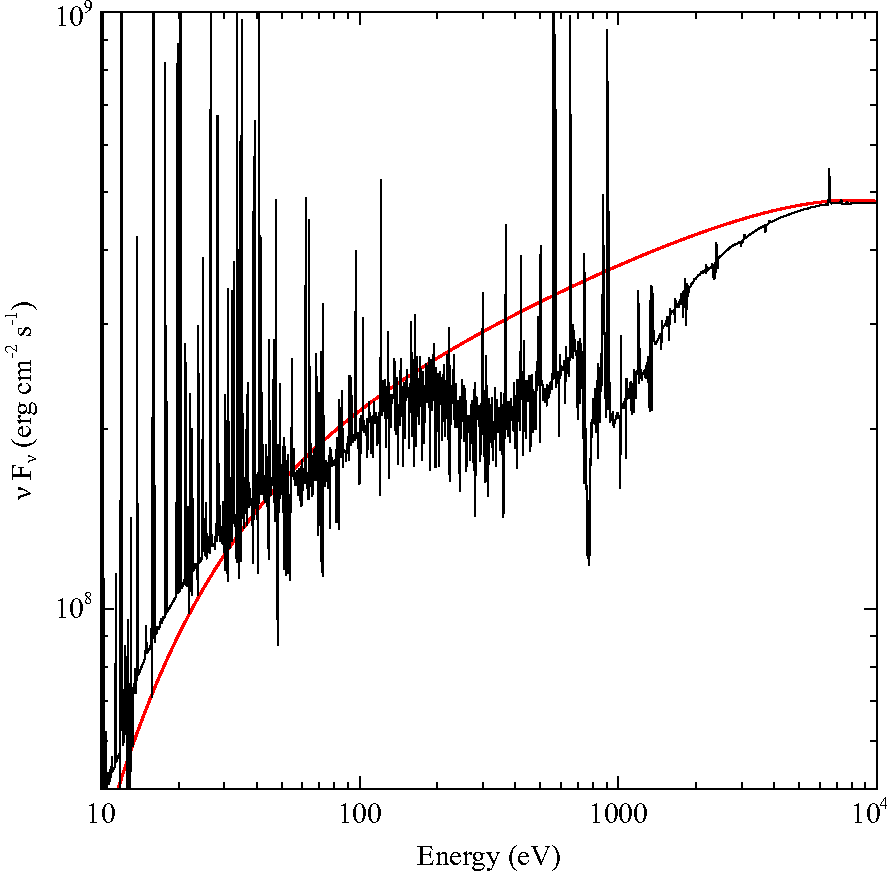
\includegraphics[scale=0.9]{WarmAbsorberReynoldsFabian}
\caption[Incident and net emission]{
\label{fig:WarmAbsorberReynoldsFabian}
The predicted X-ray spectrum of a warm absorber 
in an Active Galactic Nucleus. Prominent emission and absorption lines are present along with broad 
UTA absorption features. The parameters are from Reynolds \& Fabian (1995, MNRAS, 273, 1167).}
\end{centering}
\end{figure}

\subsection{Emission line -- continuum contrast}

In a real spectrometer the line-to-continuum contrast
depends on the spectrometer resolution if a line is unresolved.
The higher the resolution, the higher the line will appear in the spectrum.
In \Cloudy, lines are  unresolved on the coarse continuum mesh that is reported
in most versions of the \cdCommand{save continuum} command.
\Cloudy\ adds the emission-line intensities into the continuum, including the resolving power,
using Equation \ref{eqn:LineContinuumContrastFactor}.

When you plot the SED that is reported by a \cdCommand{save continuum}
command, emission lines will appear to have a triangular shape (assuming they
are not blended with lines in adjacent cells). We will treat this triangular
shape as the unresolved line profile. The total flux in that line will then be
given by the integral over this line profile, i.e. the area of the triangle.
This implies that when you perform an integral over the spectrum (e.g. to do
synthetic photometry) the line fluxes will automatically be included correctly
in the integral.

Real spectrometers may have significantly higher or lower resolution than 
\Cloudy 's coarse continuum.
The \cdCommand{set save line width / resolution} command,
described on page \pageref{sec:CommandSetSaveLWidth}, 
changes the lines relative to the continuum to make the spectrum
look like that observed with a spectrometer with a resolution that is different
from the coarse continuum.
Changing the velocity width with the
\cdCommand{set save line width} command  
has the same effect as changing the 
velocity resolution of a spectrometer measuring an unresolved line.
Smaller velocity widths will make the line rise higher above the continuum,
as shown in Equation \ref{eqn:LineContinuumContrastFactor}.
Alternatively you can also use the \cdCommand{set save resolution}
command to specify the spectral resolution of a spectrograph. Higher
values for the resolution will make the line rise higher above the continuum.

Note that this command will {\em only} adjust the height of the line, not the
width. The latter will always be the width of one cell in the coarse continuum mesh
({\em even if the line is broader than that cell}). This implies that
the line flux in the continuum array is artificially changed by the
\cdCommand{set save line width / resolution} command.
Changing the spectral resolution can be useful to emphasize weak lines in a plot,
but should never be used when energy conservation is important, e.g. when
you want to postprocess the file to fold the saved continuum with a photometric passband.

\subsection{Pumped contributions to the lines}

Continuum pumping and fluorescence are included as excitation processes
for all lines.
These contributions are usually not printed as a separate
quantity but will be if the \cdCommand{print line pump} command is entered.  Whether or not the pumped contribution actually
adds to the observed line emission depends on the geometry.
Continuum
pumping increases the line emission if no related continuum absorption is
seen by the observer.
This will be the case if the continuum source is
either not observed or not covered by absorbing gas on the observer's line
of sight.
If absorbing gas covers an observed continuum source then the
situation is like the P Cygni problem, emission produced by absorption
and pumping will not increase the total intensity of the line at~all.

The line intensity includes fluorescent excitation unless the
\cdCommand{no induced processes} command is entered.
That command is unphysical since it turns
off all induced processes.
You can judge how great the contribution of
the pumped part of the line is by printing it with the
\cdCommand{print line pump} command.

In general the treatment of scattering is very geometry dependent.
The
output produced by the \cdCommand{save continuum} commands \emph{does not} include the pumped
part of the line contribution.
This is correct if the continuum source
is included in the beam, but is not if only the gas is observed.

\subsection{Isotropic Continua}
\label{sec:save_cont_no_isotropic_option}

\par
By default the radiation field used in the calculation is reported. 
The CMB will often dominate certain portions of the spectrum,
overwhelming local emission, when it is included.
Most spectrometers in the radio and infrared will automatically remove  
isotropic emission while conducting an observation.
The \cdCommand{no isotropic} option provides a way to do a similar subtraction.
Each of the commands that set an SED shape,
described in Section~\ref{sec:IncidentContinuumShape}, will say
whether that component is isotropic or beamed.
This option will remove all sources of isotropic emission.

The commands
\cdCommand{save continuum} and
\cdCommand{save transmitted continuum}
have a \cdCommand{no isotropic} option
to not include attenuated isotropic continua in the total.
It is also possible to remove isotropic continua with the
 \cdCommand{no isotropic continua report} command described
in Section~\ref{sec:no_isotropic_continua}.

\subsection{The units option - changing the continuum units}
\label{output_units}
\label{units_option}

By default, the energy units for the first column, which gives the
wavelength or energy for each point in the continuum, are Rydbergs.  The
units can be changed to any of several energy or wavelength units with the
\cdCommand{units} keyword that appears on a \cdCommand{save continuum} command.  The following
keywords are recognized: \cdCommand{\_micron}, \cdCommand{\_eV\_}, \cdCommand{\_keV},
\cdCommand{\_MeV}, \cdCommand{wavenumber}, \cdCommand{centimeter} (also
\cdCommand{\_cm\_}), \cdCommand{\_mm\_}, \cdCommand{\_nm\_}, \cdCommand{Angstrom},
\cdCommand{\_Hz\_},\cdCommand{\_kHz}, \cdCommand{\_MHz}, \cdCommand{\_GHz},
\cdCommand{Kelvin} (also \cdCommand{\_K\_}), \cdCommand{erg\_}, and
\cdCommand{\_Rydberg}.
Both the keyword \cdCommand{units} and one of
these units must appear for the units of the energy scale to be changed.

\subsection{Save continuum uses vacuum wavelengths}
Vacuum wavelengths are always used in \cdCommand{save continuum} output.
This is to avoid a discontinuity at 2000\AA, the point where line wavelengths switch from
vacuum to air.
The \cdCommand{print line vacuum} command, 
described in Section~\ref{sec:CommandPrintVacuum},
controls whether line wavelengths
are given in air or vacuum, has no effect on \cdCommand{save continuum} output.

\subsection{Units of the save output in intensity and luminosity cases}
The units of the predicted continuum depend on whether the intensity
or luminosity case is used.
In the intensity
case continua are given as the intensity per octave
$ 4\pi \,\nu J_\nu [\ergpscmps ]$.
In the luminosity case they are
$\nu L_\nu$
[$\ergps $].
The emission from the cloud includes a covering factor if one was specified.

Through C13, the \cdCommand{save continuum} output 
in the luminosity case was per unit
cloud area at the inner radius rather than the true luminosity,
and so had units $\ergpscmps$.
This was to avoid processor limits on older computers.
Beginning in C16 output is in true luminosity units, $\nu L_\nu$, in the luminosity case.
The old behavior will the used if the
\cdCommand{set save luminosity old} option, described in
Section~\ref{sec:SetSaveLuminosity}, is used.
This is to provide backwards compatibility.

\subsection{Save continuum}

The \cdCommand{save continuum} command,
with no other keywords,
produces a file
with the following information.
The different contributors to the continuum
are defined in the Chapter \cdSectionTitle{Definitions}.

\begin{description}
\item[Column 1.]  The first column gives the photon energy in the units set
with the \cdCommand{units} option.  The default
units are Rydbergs.

\item[Column 2.]  This is the incident continuum at the illuminated face of
the cloud.

\item[Column 3.]  This is the transmitted incident continuum and does not include
diffuse emission from the cloud.
The cloud is assumed to fully cover the continuum source along our sight line, so a covering
factor has no effect.
If the option \cdCommand{no isotropic} has been issued, the transmitted continuum
does not include contributions from isotropic incident radiation sources.

\item[Column 4.]  This is the outward portion of the emitted continuum and line
emission.  This includes a covering factor if one was specified.
This does not include
the attenuated or reflected portions of the incident continuum.

\item[Column 5.]  This gives the net transmitted continuum,
the sum of the
attenuated incident (column 3) and diffuse (column 4) continua and lines.
This would be the observed continuum if the continuum source were viewed
through the gas.  Emission from the cloud includes a covering factor if one was specified.
If the option \cdCommand{no isotropic} has been issued, the net transmitted continuum
does not include contributions from isotropic incident radiation sources.
This is the same as Column 2 of the \cdCommand{save transmitted continuum} command,
described in Section \ref{sec:CommandSaveTransmittedContinuum}.

\item[Column 6.]  This is the reflected continuum
and is only predicted for an open geometry.

\item[Column 7.]  This is the total, the sum of the transmitted and reflected continua
and lines.  The attenuated incident continuum is included.
If the option \cdCommand{no isotropic} has been issued, the total continuum
does not include contributions from isotropic incident radiation sources.

\item[Column 8.] The sum of all reflected line emission.

\item[Column 9.] The sum of all outward line emission.

\item[Column 10 and 11.]  Line and continuum labels indicate the lines and
continuum edges that might contribute at that energy.  The line label gives the
label for the strongest line in the total spectrum (reflected plus outward) 
the line-center of which lies in that bin. 
(This is new in C10.  All previous versions simply reported the first line 
encountered, as is still the case with the continuum label.)   
The continuum labels are established when the code
is set up and they do not mean that the continuum feature is actually
present in the spectrum.  

\item[Column 12.]  This gives the number of emission lines within that continuum
bin, divided by the ratio of the energy width of the cell to the cell's
central energy, $dE/E$.  So this is the number of lines per unit relative
energy.
\end{description}

\noindent
This command will save the continuum at the outer edge of the cloud unless the
keyword \cdCommand{every} appears on the command line, in which case it will
save the continuum for every zone.

\subsection{What is observed}

Figure \ref{fig:EmissionSaveComponents} illustrates several
possible geometries.
Two lines of sight to the central object are shown,
and two clouds are shown.
Each cloud produces both a reflected and transmitted emission component.

\begin{figure}
\centering
\begin{centering}
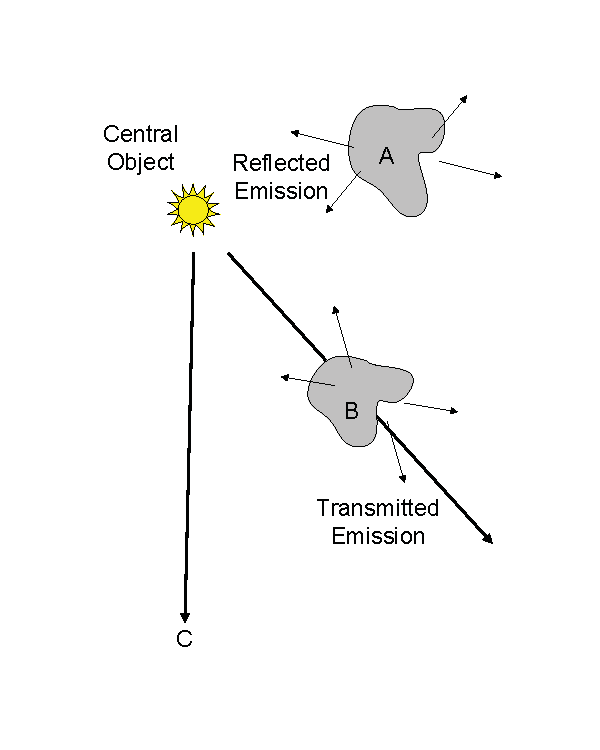
\includegraphics[scale=0.9]{EmissionSaveComponents}
\caption[Radiation field components in save continuum]{
\label{fig:EmissionSaveComponents}
This figure illustrates several components of the radiation field that enter in
the calculations.}
\end{centering}
\end{figure}

Three possible geometries, indicated by the letter on the figure, occur
depending on how we view the central source and clouds: a) we do not directly
observe the central object although we may see it by reflection from the
illuminated face of a cloud, b) we observe the transmitted continuum and
the outward emission from the emitting cloud, and c) we observe the
unattenuated continuum directly without absorption.
Column 2 gives the
unattenuated continuum, and column 3 gives the attenuated continuum.

There are also three possible situations for the line emission.
First,
we might only observe clouds that lie on the near side of the continuum
source.
In this case we see the ``outward'' line emission.
Second, we
might only observe clouds that lie on the far side of the continuum source.
In this case we only see the ``reflected'' or inward component.
Lastly,
we might observe a symmetric geometry with reflected emission from the far
side and outward emission from the near side.

In most cases an observer at large distance from the structure would
observe \emph{both} the central object and the cloud and would measure the quantity
listed in column 5 (if only transmitted emission is detected) or column
7 (if both reflected and transmitted continua are seen).  If the central
object is not seen then the quantity in column 4 would be observed.

\subsection{Save continuum bins}

This saves the continuum energy bins.
The first column is the center
of the bin in whatever unit was set after the \cdCommand{units} keyword
(see Section~\ref{units_option} for details).
The second column is also the center of the bin, but this time always in Ryd.
The third column is the cell width $\delta\nu$, also in Ryd.
The bin extends from $\nu-\delta\nu/2$ to $\nu+\delta\nu/2$.

\subsection{Save cumulative continuum}
\label{sec:CommandSaveCumulativeContinuum}

This gives the continuum integrated over a time-dependent simulation.
The usual \cdCommand{save continuum} command gives the
continuum for the current time step in these calculations.
The units of the usual \cdCommand{save continuum} command
are flux per octave, $\nu f_{\nu}\; [\ergpscmps ]$.
This command gives the time-integrated energy,
$\nu E_{\nu}\; [\ergpscm ]$.

\par
Note that using this command with the option \cdCommand{no isotropic}
will cause \Cloudy\ to exit immediately with an error message.

\subsection{Save diffuse continuum}

This reports the local diffuse line and continuous emission
coefficient $4 \pi \nu j_{\nu}$ [\ergpccmps ].
Optical depth effects are not included.

By default this reports the diffuse emission from the last zone.
The first column of the output gives
the photon energy including the \cdCommand{units} option.
The second column gives the diffuse continuous emission.
The third column gives the line emission in the same units,
including the effects of the
\cdCommand{set save line width / resolution} command described on page
\pageref{sec:CommandSetSaveLWidth} when appropriate.
The last column gives the total.

If the keyword \cdCommand{zone} appears then the diffuse emission
\emph{from every zone} will be reported.
The first row gives the wavelength or energy scale.
The remaining rows give the total (line and continuum)
emission coefficients $4 \pi \nu j_{\nu}$
at each energy.

\subsection{Save continuum emissivity 12 [units micron]}

This command will save the continuum volume emissivity $4\pi \nu j_\nu$ (in
\ergpccmps), as well as the local absorption and scattering opacity (in
cm$^{-1}$) as a function of radius and depth (in cm). This output can be used by an
external program to do more specialized radiative transfer, e.g.\ to determine
the continuum flux through an aperture. To make this process second-order
accurate, the radius and depth in the middle of each zone is reported. One number should
be supplied on the command line, which is the wavelength / frequency at which
the emissivity and opacity will be evaluated. You can use the keyword
\cdCommand{units} as described in Section~\ref{output_units}. By default the
frequency is assumed to be in Rydberg.

\subsection{Save emitted continuum}

The continuum emitted and reflected from the nebula is saved.
The
first column is the photon energy.
The second column is the reflected
spectrum.
The third column is the outward diffuse emission.
The fourth
column is the total emission (the sum of the inward and outward emission).
This would be the observed emission from the nebula if the central continuum
source was not in the beam but clouds uniformly cover the continuum source.
The last two columns are labels for lines and continua contributing at each
energy.
The attenuated incident continuum is not included in any of these
components.
The effects of a covering factor are included.
The continua have units
$\nu f_{\nu}$ [\ergpscmps ] or $\nu L_{\nu}$ [\ergps ] 
depending on whether the intensity or luminosity case is specified.

\subsection{Save fine continuum [range, merge]}

The code transfers the continuum on a coarse mesh, needed for speed in
evaluating photo-interaction rates, and on a fine mesh, needed for automatic
treatment of line overlap.
The coarse continuum is the one given in output
from the \cdCommand{save continuum} command and it includes all the components shown in Figure \ref{fig:EmissionSaveComponents}.
The fine continuum is designed to account for line transfer.
It shows a normalized attenuated incident continuum and 
does not include continuous
emission or absorption from the cloud.  
This multi-grid approach is needed to combine precision and speed.

This command reports the energy (see below) of the fine continuum bin in the
first column, and the continuum transmission coefficient,
$I_{transmitted}/I_{incident}$, for the fine continuum in the second column.
What follows is a list of absorption lines centered on that energy bin.
Each line is identified by its spectral label (species and wavelength), and is
followed by its mean optical depth.
The latter is the same as the last entry reported by
\cdCommand{print line optical depths}, see Section \ref{sec:PrintLineOptDep}.
All lines centered on that bin are reported, sorted from most-to-least opaque.

The resulting output will be huge if the entire fine continuum is saved.
{\it Users are advised to make use of the {\rm\cdCommand{range}} option
to limit the size of the output file.}
If the keyword \cdCommand{range} appears then
the lower and upper limits to the range
of the fine continuum must be entered.
The command also accepts
a \cdCommand{units} option,
described on page \pageref{output_units}, to change the units used
in the specified energy range, and in resulting output.

The optional third numerical parameter gives the number
of fine continuum cells to average together, again with the intent of
reducing the size of the output file.  The default is to average over 10
cells.  If the number of cells to be combined is specified then it must
be the third number on the command line, following the limits
of the range.
Note that in a given energy range, the same number of features is reported,
irrespective of the number of cells merged.

The resolving power of the fine continuum is adjusted when the calculation begins so
that lines of the heavy elements can be resolved.
The resolving power is reported in the main printout with the string
\cdCommand{R(F~Con)}.

\subsection{Save grain continuum}

The thermal emission by grains is part of the emergent continuum.  This
command saves only the grain emission in the optically thin limit for
the last zone.  It is mainly intended as a debugging aid.

The first column gives the photon energy in the units specified with
the \cdCommand{units} option.  The second column gives the total emission from
carbonaceous grains (including amorphous carbon and PAH's).  The third column
gives all emission from all constituents that are not carbonaceous.  In
practice this will be mainly the silicates.  The last column gives the sum
of the two.

\subsection{Save incident continuum}
\label{sec:CommandSaveIncidentContinuum}

The incident continuum, that emitted by the central object and striking
the illuminated face of the cloud, will be saved.  The first two columns give
the photon energy and the continuum specific intensity 
$\nu 4\pi J_{\nu}$ [erg cm$^{-2}\ \mathrm{s}^{-1}$] 
or specific luminosity 
$\nu L_{\nu}$ [erg  $\mathrm{s}^{-1}$].
The photon occupation number 
\begin{equation}
{\eta _\nu } \equiv {J_\nu }\left( \nu  \right)\,{\left( {\frac{{2h{\nu
^3}}}{{{c^2}}}} \right)^{ - 1}}
\end{equation}
concludes the line.

\subsection{Save interactive continuum}

This gives the product of the internal radiation field times the gas opacity integrated over the full continuum.  
The results are produced for each zone and give
the attenuated incident continuum, the OTS line, the OTS continuum, the
outward continuum and the outward lines.  The first optional number is the
lowest energy in the output.  If missing or zero, the lowest energy
considered by the code will be used.  Numbers less than 100 are interpreted
as the energy in Rydbergs and those greater than 100 as the cell number.

\subsection{Save ionizing continuum [options]}

This creates a file that can be used to indicate ionization sources.
If the keyword \cdCommand{every} occurs then this is saved for every zone, otherwise
it is only saved for the last zone.

The first optional number on the command line is the lowest energy to
include in the output.  If it is missing or zero then the lowest energy
considered by the code will be used.  It is interpreted as the energy in
Rydbergs if the number is less than 100 and as the cell number if it is
greater than 100.  The second optional number is the threshold for the
faintest interaction to print.  The default is one percent of the quantity
given in the \cdMono{rate/tot} column.
Enter zero for this number if you want
all interactions to be printed.  The optional numbers may be omitted from
right to left.

The first column in the resulting output is the cell number
of the C scale, so the first cell is zero.
Next comes the photon energy
in Rydbergs unless changed with the \cdCommand{units} option.  The third column, with
the header \cdMono{flux}, is the flux of photons within this frequency bin
(\emph{not}
per unit frequency) with units s$^{-1}$~cm$^{-2}$.  The forth column gives the
photo-interaction rate, the product of the flux multiplied by the gas
absorption cross section
[cm$^{-2}$] and so with units s$^{-1}$.  The next five numbers are the fractions of
this photo-interaction rate due to the attenuated incident continuum, the
OTS line, the OTS continuum radiation fields, and the outward lines and
continua.  The 10$^{\mathrm{th}}$ column, with the heading \cdMono{rate/tot}, is the ratio
of this photo rate to the total integrated radiation-field interaction rate.
The next column, with the heading \cdMono{integral}, is the integrated cumulative
interaction, the integral of the previous column over energy.  This makes
it easy to identify the portions of the radiation field that have the
dominant interaction with the gas.  The last two labels on the line indicate
which lines and continua contribute at that energy.

\subsection{Save raw continuum}

This saves the \cdTerm{raw} continua.
This is exactly the continuum used
within the code.  The first number is the photon energy.  The next columns
are the contents of many of the continuum arrays at each energy.  Consult
the source to see which arrays are now saved.  Each gives the number of
photons stored in that cell with units photons s$^{-1}$ cm$^{-2}$
cell$^{-1}$.  The last
number is the number of lines within that cell.

\subsection{Save reflected continuum}

The reflected continuum is output if \cdCommand{sphere} is not set.  The first column
is the photon energy, the second the reflected continuum $4\pi \,\nu J_\nu
$ [erg  cm$^{-2}$~s$^{-1}$] at that energy.  The third gives the reflected lines
and the fourth is the sum of these two.  Someone who could only see the
illuminated face of the cloud would observe this.  The next column is the
effective albedo of the cloud, the ratio of the reflected to incident
continuum (the \cdCommand{save total opacity} command will give the
true albedo).  The last column gives the label
for continuum processes with thresholds at each energy.

\subsection{Save transmitted continuum [no isotropic]}
\label{sec:CommandSaveTransmittedContinuum}

This saves the transmitted spectrum (i.e., the attenuated incident SED and the outward component
of the diffuse continuum and line emission) predicted at the end of the calculation.
It is affected by the \cdCommand{no isotropic} option.
The data are the same as Column 5 of the \cdCommand{save continuum}
command described in Section \ref{sec:CommandSaveContinuum}.

This save file can be used as part of the incident continuum in a later
calculation by reading it with the \cdCommand{table read} command described in
Section~\ref{sec:CommandTableRead}.

The code will implicitly behave as if the keyword \cdCommand{last} had been
included. This is needed since the code would become confused if it tried to
read a file containing information from multiple iterations. So the output
would be useless without this keyword. In a grid run it will also implicitly
save the continuum into a separate file for each grid point. This is needed
for the same reason: the code cannot read a concatenated output file.

Two cautions apply when reading this file as an input continuum. First, save
output should not be written into the same file as the input file during the
second calculation. The file containing the first continuum will be
overwritten if this occurs. Second, the first couple of lines contain header
information that is needed by the code. They should not be deleted.

This command is unusual in that it always saves the SED in intensity units,
even when the simulation is done in luminosity mode. If the radius is set, the
continuum will be an intensity normalized at the outer radius. If the radius
is not set, the intensities will have the usual normalization also used in
other \cdCommand{save continuum} commands.

The line-to-continuum contrast factor \cdVariable{Resolution}
set by the \cdCommand{set save line width / resolution} command
(see page \pageref{sec:CommandSetSaveLWidth})
is not used in this command.  This is to insure that lines have
the correct intensity in the save file, as needed for energy conservation.
The \cdCommand{units} keyword is also ignored. The output will always use
the standard unit (Rydberg) as the frequency unit.

\subsection{Save two photon continuum}

This saves the total two-photon continuum and is mainly a debugging
aid.  The photon energy is followed by the number of photons emitted per
Rydberg per second, then by $\nu F_\nu$.  The details of two photon emission,
including induced processes, are discussed by \citet{Bottorff2006}.

\section{Save convergence [reason, error]}

These commands produce information about various aspects of the converged
solution.

\subsection{Save convergence base}

The gives computed values of many quantities that are converged during
a calculation.  The values are given as they are at the exit to the base
convergence routine.  Depending on the convergence properties of the
solution, there will be between only a few up to many
dozens of evaluations in each zone.

\subsection{Save convergence error}

This will produce information concerning the quality of the converged
pressure, electron density, and heating-cooling solution.  The correct value,
converged value, and percentage error, (correct-converged) $\times$ (100/correct), will be produced for each zone.

\subsection{Save convergence reason}

This will save the reason the model was declared ``not converged'' at
the end of each iteration when the
\cdCommand{iterate to convergence} command is used.

\section{Save cooling}

This saves the cooling agents for each zone.  The first number is the
depth [cm] followed by the temperature [K].  The next two numbers are the
total heating and cooling rates [erg cm$^{-3}$~s$^{-1}$], not including
advective terms; advective cooling is reported separately in the fifth column.
The remaining labels indicate contributors to the cooling array and the
fraction of the total cooling (ignoring advective cooling) carried by that agent.
At least four (4) agents are reported, or more if they are ``bright'' enough.
The faintest coolant saved is normally 0.05 of the total (sans advective),
and can be reset with the \cdCommand{set WeakHeatCool} command.

This is mainly used for debugging and its output is not well documented.
The line labels may, or may not, correspond to labels used in the main
emission-line output.  The code adds individual coolants to the total cooling
by calling routine \cdRoutine{CoolAdd}.
The arguments to that call include the string
and a number that follows it.   To discover the process for a particular
label you will need to search over the entire code to find where that string
occurs in a call to \cdRoutine{CoolAdd}.
The string will be within a pair of double
quotes.
As an example, two coolants that might appear are
\cdTerm{dust 0}, and \cdTerm{H2cX 0}.  A search on the string \cdMono{"H2cX"} (include the beginning and ending double
quotes) will find the string occurring in two places, where the cooling
is added with the call to \cdRoutine{CoolAdd} and another place where the cooling itself
is evaluated.  Comments around the call to \cdRoutine{CoolAdd}
indicate that \cdTerm{H2xC} is
cooling due to collisional excitation within the ground electronic state
of \htwo.   A search on the string \cdMono{"dust"} finds its call to
\cdRoutine{CoolAdd} with
the comment that it is cooling due to grain recombination cooling.

Cooling due to the unified iso-electronic sequences is different since
the label that occurs in the call to \cdRoutine{CoolAdd} is generated by the routine
that evaluates the cooling and does not explicitly occur in the source.
The iso-electronic cooling labels begin with \cdMono{"IS"},
followed by a string
indicating the process, and followed by strings giving the iso-electronic
sequence and the element.  Search for the start of the string but not for
the element name.  An example might be the string
\cdMono{"IScionH H"}.  The \cdMono{"IS}
indicates that it is cooling due to an ion along the iso-electronic sequences
and the two ending H's indicate that the coolant is H-like hydrogen.  The
string \cdMono{"IScion"} occurs in the source and comments indicate that the process
is collisional ionization cooling.  The iso-electronic cooling strings do
not include a pair of double quotes in the source since the ending double
quote occurs after the element names.  You would search for the string
\cdMono{"IScion"}.

\subsection{Save cooling each}

If keyword \cdCommand{each} appear after \cdCommand{save cooling}
command, the cooling of each element and for certain
special cases will be saved for each zone. 
The unit of the cooling rate is [erg cm$^{-3}$~s$^{-1}$]. 
Notice that the output metal bremsstrahlung cooling is the real 
metal bremsstrahlung cooling minus the total bremsstrahlung heating. If the
bremsstrahlung heating is comparable with the real metal bremsstrahlung cooling,
the output may not be precise.
The cooling due to molecules is listed separately. The total cooling
listed in column 3 does not include the dynamics cooling (adve, column 45).

\section{Save charge transfer}

Charge transfer recombination and ionization rate coefficients
   [cm$^3\mathrm{s}^{-1}$]
for hydrogen onto heavier elements will be output.  The rates will be
evaluated at the temperature of the last computed zone.  Rates for
recombination (${\mathrm{A}}^{ + x}  + {\mathrm{H}}\to{\mathrm{A}}^{ + x + 1}  + {\mathrm{H}}^
+$) are first, followed by the rates for the opposite ionization process.
The first number is the atomic number of the species.

\section{Save Chianti}
\label{sec:CommandSaveChianti}

This saves collision strengths for Chianti transitions over a certain temperature range.
The output gives species, lower level, upper level, wavelength in Angstroms, 
and collision strengths for each temperature given in the header row.
This reports data for all active Chianti species in that particular run.

\section{Save dr}

The logic behind the choice of zone thickness will be described.

\section{Save dt}

The logic behind the choice of time step in time-dependent simulations will be described.

\section{Save dynamics options}

This produces some information concerning the dynamics solutions.

\subsection{Save dynamics advection}

This produces information about advection terms.

\section{Save element \emph{name}}

This will save the ionization structure of any element. The output will
have one line per zone giving the ion fraction\footnote{Before version 96 the ionization fractions only included atoms and
ions.  They now include molecules.  The sum of the atomic and ionic fractions
will not add up to unity if a significant fraction of the element is in
molecules.} of each successive stage
of ionization.  The keyword \cdCommand{element} must be followed by the element name.

The first number on the resulting output is the depth [cm] into the cloud.
The remaining lines give the relative ionization fraction of the $n+1$ possible
stages of ionization where $n$ is the atomic number of the element.  These
may be followed by some of the more abundance molecules.

If the keyword \cdCommand{density} appears on the command line then the
density [cm$^{-3}$]
will be given rather than the dimensionless fraction.

\section{Save enthalpy}

The file will list the depth into the cloud, followed by the total
enthalpy, and various contributors to it.

\section{Save execution times}

The code will output the zone number, the time required to compute that
zone, and the elapsed time since the start of the calculation.  This is
intended as a mechanism to identify zones that require large amounts of
work to converge.  
This command is being superseded by the \cdCommand{save performance} command.

\section{Save FeII}
\label{sec:CommandSaveFeII}

These commands are obsolete.
See the \cdCommand{save species} family of commands,
Section~\ref{sec:SaveSpecies}.

\section{Save FITS}

This command produces photon energies and the total transmitted continuum into
a two-column file in FITS (Flexible Image Transport System) format.  FITS
is a standard format used in astronomy, and endorsed by both NASA and the
International Astronomical Union.  The most current definition of the FITS
format is by \citet{Hanisch2001}.  This was added by Ryan Porter and its
first application is given in \citet{Porter2006}.  The saved spectrum will
by default include the isotropic continua.  They can be excluded using the
\cdCommand{no isotropic continua report} command.  The saved spectrum will
always conserve energy, i.e. the \cdCommand{set save resolving power} command
has no effect.

Since only one spectrum can be stored in a FITS file, the command will
implicitly behave as if the keyword \cdCommand{last} was included on the
command line.

The following creates a FITS file with a blackbody continuum
\begin{verbatim}
blackbody 1e5 K
ionization parameter -2
save FITS "filename"
\end{verbatim}

This command is often used with the \cdCommand{grid} command which creates
grids of calculations. In this case, the command produces separate FITS files
for each grid point. They will have names
\cdFilename{grid000000000\_filename}, \cdFilename{grid000000001\_filename},
etc., where \cdFilename{filename} is the file name you supplied between double
quotes. The meaning of the grid index embedded in the filename can be found with
the \cdCommand{save grid} command described in Section~\ref{sec:save:grid}.

\section{Save gammas}

This gives the photoionization rates for all subshells of all ions for
the last zone.  The numbers are the element, ion, and subshell numbers,
followed by the photoionization and heating rates from that subshell.  The
remaining numbers are the fractional electron Auger yields.

\subsection{Save gammas element oxygen 1}

If the \cdCommand{element} keyword appears then the detailed contributors to the
photoionization rate for the valence shell of a particular element will
be produced by calling \cdRoutine{GammaPrt}.
The ionization stage must also appear,
with 1 the atom, 2 the first ion, etc.

\section{Save Gaunt factors}

This produces a series of tables showing the thermally averaged free-free
Gaunt factors as a function of the log of the photon energy (vertical, in Ryd)
and the log of the electron temperature (horizontal, in K). Such a table is
produced for each charge state treated by \Cloudy. Below each table, the Gaunt
factors are repeated as triplets, but this time as a function of the customary
dimensionless units $\log \gamma^2$ and $\log u$ rather than temperature and
photon energy.

\section{Save grains [options]}

These commands give grain properties.  Several grain species are usually
included in a calculation.   Often there are several size bins per grain
type.  These commands will print a line giving a list of the grain labels,
followed by a line giving the grain radius in $\mu m$.
The following lines then give the individual grain properties
(temperature, potential, etc) for each size and type.

Details of the grain physics are given in \citet{Baldwin1991},
\citet{Weingartner2001a},
\citet{VanHoof2004}, and \citet{Weingartner2006}.

\subsection{Save grain abundance}

The grain abundance [g cm$^{-3}$] for each grain bin and the total grain
abundance is given as a function of depth.

\subsection{Save grain charge}

The first number is the electron density [cm$^{-3}$] contributed by grains.
A positive number indicates that grains where a net source of electrons
so they have a net positive charge.  The remaining columns print the charge
of each grain size and type, in number of elementary charges per grain,
for each zone.

\subsection{Save grain continuum}

This is listed in the \cdSectionTitle{save continuum} section.

\subsection{Save grain D/G ratio}

The dimensionless dust to gas ratio for each grain bin and the total
grain abundance is given as a function of depth.

\subsection{Save grain drift velocity}

The drift velocity [km s$^{-1}$] of each grain species is printed for each zone.

\subsection{Save grain extinction}

The grain extinction at the $V$ filter will be saved as a function of
depth.  This extinction only includes grains, although they should provide
nearly all the extinction when they are present.  The first column gives
the depth into the cloud [cm], the second is the extinction [mag] at the
$V$ filter for an extended source, like a PDR, and the third number is the
extinction for a point source like a star.  This distinction is discussed
in Sections 7.2 and 7.6 of AGN3.  The extended source extinction discounts
forward scattering by writing the scattering opacity as $\sigma ( 1-g )$,
where $\sigma$ is the total scattering opacity and $g$ is the grain asymmetry
factor.
The quantity in the last column does not include the $({1-g})$
term.

\subsection{Save grain H2rate}

The grain \htwo\ formation rate is given for each size and type of grain
and for each zone.

\subsection{Save grain heating}

The grain heating [erg cm$^{-3} \mathrm{s}^{-1}$] is output for each zone.

\subsection{Save grain opacity}

This gives the grain opacity as a function of the photon energy in the last
zone of the model.  The first column is the photon energy in the units set
with the \cdCommand{units} option, the second the total (absorption plus
scattering) cross section, followed by the absorption and scattering cross
sections.  These are the summed cross section per proton for all grain
species in the calculation. Column 5 is the pure scattering cross section
summed over all grains and column 6 is the grain albedo.   Columns 2, 4,
and 6 use the scattering cross section multiplied by $(1-g)$, while column
5 does not. The opacities have units [cm$^{2}$ H$^{-1}$] using the actual
grain abundance from the last zone.

\subsection{Save grain potential}

 The grain floating potential [eV] is output for each grain size bin and
each zone. The grain potential is defined~as
\begin{equation}
\varphi _g  = \frac{{\left( {\left\langle Z \right\rangle  + 1} \right)e^2
}}{a}
\end{equation}
where $\langle Z\rangle$ is the average grain charge of the grain size bin.  In reality
there is a distribution of grain charges in each bin, so this quantity does
not relate to any individual grain. It is approximately the amount of energy
needed to move an electron from the grain surface (after it has been lifted
out of the grain potential well) to infinity, averaged over all charge
states.
\citet{Weingartner2001a}, \citet{VanHoof2004} and \citet{Weingartner2006} provide further details.

The grain potential given here and the (average) grain charge
(see \cdCommand{save grain charge}) differ only by constants.  It
is probably best to use the latter since that quantity will be far easier
to define. Refer to \citet{Weingartner2001a} and
\citet{VanHoof2004}
for more details.

\subsection{Save grain qs}

The photon energy in Rydberg is followed by the absorption and scattering
efficiency for each grain species. The absorption efficiency $Q_{\rm abs}$ is
defined as the ratio of the absorption cross section $\sigma_{\rm abs}$ and
the geometric projected grain surface area $\sigma_{\rm g} = \pi a^2$. This
yields: $Q_{\rm abs} = \sigma_{\rm abs}/\sigma_{\rm g}$. A similar definition
holds for the scattering efficiency, keeping in mind that the scattering cross
section has been multiplied by $(1-g)$, i.e., we print: $Q_{\rm scat} (1-g) =
\sigma_{\rm scat} (1-g) / \sigma_{\rm g}$. See also Chapter 7 of AGN3.

\subsection{Save grain temperature}

The temperature of each grain species is printed for each zone.

\section{Save grid}
\label{sec:save:grid}

This is used with the \cdCommand{grid} command to
create a file giving the parameters for each simulation in a large grid
of calculations.  This can be combined with other \cdCommand{save} commands to create
files giving the derived quantities for a large set of calculations.

The first row gives tab-separated column titles.  The column title for the parameters
that are varied will give the first few characters of the command line for
that parameter.  Each of the following lines summarizes a particular grid point.  The
first column gives the index number in the grid. This is useful if you
have separate output for each grid point (e.g. from the \cdCommand{save FITS}
command). The index number will be part of the file name in that case. It is
also useful for finding back the output from a particular grid point in a
save file (see Section~\ref{sec:GridOutputOptions} for more details).
The next two columns indicate whether the calculation had a failure or had any
warnings.  A successful calculation will have ``F'' (for false) indicating
no failure or warning occurred.  If either of these is ``T'' (for true) then
that simulation had major problems. The following column is a string giving
a bit more detail about the exit code. It says ``ok'' if everything went fine
and ``warnings'' if warnings were present in the run, but nothing more serious.
If the simulation failed completely, you could see strings like ``cloudy abort''
or ``early termination''. You should look at the detailed output
to find out what went wrong. The next two columns give the number of the
MPI rank that executed the simulation (will be zero in non-MPI runs) and the sequence
number of the simulation on that rank (they are executed in random order). These
numbers are used for debugging the code. The next columns give numerical parameters for
each simulation in the grid.  The last column gives all the grid parameters
as a single string.  Many plotting programs will allow you to add this string
next to each of the plotted data points.

This command does not produce any output if the \cdCommand{grid} command
is not used. In grid runs it is highly recommended to always include this command.
It allows you to see in one glance if the run was successful and where the problems
are in case it was not. It is also useful to include this output in case you want
to file a bug report.

\section{Save heating}

The code will save the heating agents for each zone.  The first two columns
give the depth [cm] and temperature [K].  The next two columns give the
total heating and cooling rates [erg cm$^{-3}$~s$^{-1}$], not including
advective terms; advective heating is reported separately in the fifth column.
This is followed by a set of labels for various heat sources and the fraction
of the total heating (ignoring advective heating) carried by that agent.
At least four (4) agents are reported, or more if they are ``bright'' enough.
The faintest agent saved is normally 0.05 of the total (sans advective), and
can be reset with the \cdCommand{set WeakHeatCool} command.

The heating labels will probably not correspond to any entries in the
emission-line list.  If the identification of a heat source is in question
the best recourse is to search for the heating label over the entire code.

\section{Save [option] history}

\subsection{Save pressure history}

This follows the pressure and density convergence history.

\subsection{Save temperature history}

This follows the temperature and heating---cooling convergence history.

\section{Save H2}

Some details of the large \htwo\ molecule are output as a save file.  One
of the following options must appear.  The large \htwo\ model is not enabled
by default but is turned on with the \cdCommand{database H2} command.

Many studies of \htwo\ properties will use plots showing populations as a
function of excitation energy.  The slope gives a population temperature,
which may be related to the kinetic temperature under some circumstances.
Theoretical plots can be made using the
\cdCommand{save H2 column density}
or \cdCommand{save H2 populations} commands described below.
The level energy in K, given in
the save output, is the x-axis and the column density or population in
each level is the y-axis.

The \cdCommand{save grain H2rate} command gives
the \htwo\ formation rate for each of the grain species included in the calculation.

\subsection{Save H2 column density}

This saves the column density of ro-vibrational states within the ground
electronic state.  This command recognizes the same options as the \cdCommand{save H2 populations} command.

The file begins with the total \htwo\ column densities
in the ortho and para forms, followed by the total \htwo\ column density.  The remainder of the file
gives the $v$ and $J$ quantum indices, followed by the excitation energy of
the level in K, the total column density in that level, and finally the
column density divided by the statistical weight of the level.

\subsection{Save H2 cooling}

This produces a file containing heating and cooling rates
[$\pcc\ \ps$] as a function of depth.

\subsection{Save H2 cooling per molecule}

This produces a file containing the LTE cooling (for transitions within the X band only),
and the net H2 cooling (cooling minus heating) as a function of temperature.
Each measure of cooling is reported per H2 molecule in units of \ergps.

\subsection{Save H2 creation}

This command has been superseded by the \cdCommand{save chemistry rates} command.

\subsection{Save H2 destruction}

This command has been superseded by the \cdCommand{save chemistry rates} command.

\subsection{Save H2 heating}

This produces a file containing the depth, total heating rate [erg
cm$^{-3}\mathrm{s}^{-1}$], and \htwo\ heating predicted by an expression in \citet{Tielens1985a}, together with the heating predicted by the large model of the \htwo\ molecule.

\subsection{Save H2 levels}

This creates an energy-ordered list of the levels within X.  The first
column gives the energy in wavenumbers relative to the lowest level, the
second gives the statistical weight, and the next two columns give the
vibration and rotation quantum numbers.  The sum of the transition
probabilities is given, followed by the sum of collisional de-excitation rate
coefficients (cm$^{3}$ s$^{-1}$) of the level for each of the colliders 
included in the calculation.

\subsection{Save H2 lines}

The intensities of all significant \htwo\ emission lines that are produced
within the ground electronic configuration are given.  The file also gives the
information needed to convert an emission-line spectrum into a level
population vs excitation energy diagram.

Each line of output begins with a spectroscopic designation of the line,
followed by the upper and lower electronic, vibration, and rotation quantum
numbers.
This is followed by the wavelength of the line in microns.
The
line wavelength is then printed as it appears in the output.
The log of
the intensity or luminosity in the line (depending on whether the intensity
or luminosity case is specified), and the intensity of the line relative
to the normalization line, follow.
The excitation energy of the upper
level of the transition in Kelvin and the product
$g_u h\nu A_{ul} $  for each line are also given.
This product is needed to convert
intensities into excited-state column densities.

Only lines brighter than 10$^{-4}$ of the reference line are given by default.
The intensity of the faintest line, relative to the normalization line,
is set with the first optional number that can appear on the command line.
If the number is negative then it is interpreted as the log of the limit.

By default only lines within the ground electronic system are saved
but this can be changed if the keyword \cdCommand{electronic}
appears on the command line.
If the keyword \cdCommand{all} also appears then lines
within all electronic systems are saved.
If the keyword \cdCommand{ground} appears then only lines the
ground system are saved.  This is the default.  If a number appears then
it is the number of electronic systems to be saved, 1 for only the ground
electronic state.  If the number of systems is specified then it must be
the second number on the line---the first being
the intensity of the faintest line to print.

The following give examples.  The first sets the faintest \htwo\ line to
save.  Only lines within the ground electronic system will be produced.
\begin{verbatim}
save H2 lines, faintest -4 "filename"
\end{verbatim}
This sets the faintest line, and also requests all lines produced by all
electronic configurations.
\begin{verbatim}
save H2 lines, faintest -4 all "filename"
\end{verbatim}
This example requests only lines for the lowest three electronic
configurations.
\begin{verbatim}
save H2 lines, faintest -4 electronic 3 "filename"
\end{verbatim}

\subsection{Save H2 populations}

The level populations for the ground electronic state are given for the
last computed zone.  The populations are relative to the total \htwo\ abundance.

There are several optional parameters.
The quantum numbers of the highest
vibrational and rotational levels to save can be specified as consecutive
numbers on the command line.
These occur in the order $v$ then $J$.
If no
numbers occur, or if a limit that is less then or equal to zero is entered,
then populations of all levels will be saved.

If the keyword \cdCommand{zone} appears then the level populations 
will be saved for every zone.   These are all given along one long line,
a format that is different from the other output options.  Otherwise the
populations are only saved at the end of the iteration using the output
options described next.

If output is only saved for the last zone then it can be in either
a triplet format, with the vibration and rotation quantum numbers followed
by the population, or as a matrix, with all populations of a given vibration
quantum number lying along a single row.  The triplet form is done by
default, and the second will occur if the keyword
\cdCommand{matrix} occurs on the command line.

The \cdCommand{save H2 column densities} command provides similar output
options but for integrated column densities.

\subsection{Save H2 PDR}

The output contains six columns giving the depth (in cm), the
o-\htwo\ density, the p-\htwo\ density (both in cm$^{-3}$), and the Solomon
dissociation rate following \citet{Tielens1985a}, \citet{Bertoldi1996}, and
the \Cloudy\ big \htwo\ model, respectively (in s$^{-1}$).

\subsection{Save H2 rates}

The output contains useful information regarding \htwo\ formation and
destruction rates.

\subsection{Save H2 Solomon}

The output will give the total rate for photo-excitation from the ground
to electronic excited states and then identify those levels which are the
dominant contributor to the total rate.

\subsection{Save H2 special}

This provides infrastructure to save debugging information.  It can
be easily changed to suite particular needs.

\subsection{Save H2 temperatures}

The depth [cm], 21 cm spin temperature [K], gas kinetic temperature [K],
and several temperatures derived from relative populations of $J$ levels within
the H$_2\, v=0$ ground  electronic state [K], are saved for each zone.

\subsection{Save H2 thermal}

A variety of heating---cooling processes involving \htwo\ are given
for each zone.

\section{Save helium [options..]}

\subsection{Save helium line wavelengths}

This gives wavelengths of lines from $n=2$ levels of He-like ions.

\section{Save hydrogen}

\subsection{Save hydrogen 21 cm}

This gives some information related to the spin temperature of the 21
cm line.
The keyword is either \cdCommand{21 cm} or \cdCommand{21cm}.
The level populations
within 1s are determined including radiative excitation by \la, pumping by
the external and diffuse continua, collisions, and radiative decay.  Several
of the resulting populations and temperatures are included in the output.

\subsection{Save hydrogen conditions}

This gives the physical conditions and populations of various forms of
hydrogen are given as a function of depth.  The depth [cm], temperature
[K], hydrogen density [cm$^{-3}$], and electron density [cm$^{-3}$] are followed by
the densities of \hO, \hplus, \htwo, H$_{2^{+}}$, H$_{3^{+}}$, and H$^-$ relative to the total hydrogen
density.

\subsection{Save hydrogen ionization}

This gives rates for processes affecting the hydrogen ionization as a
function of depth.  The columns give the ground state photoionization rate
[s$^{-1}$], the total and Case~B recombination coefficients [cm$^3$~s$^{-1}$], the
predicted ratio of $n$(\hplus) to $n$(\hO), and the theoretical ratio for the simple
case.  Finally, contributors to the ground state photoionization rate are
produced with a call to \cdRoutine{GammaPrt}.

\subsection{Save hydrogen lines [alpha]}

The upper and lower quantum indices, the line wavelength, the optical
depth, and the intensity of the emitted line, will be saved. If the \cdCommand{alpha}
option is used, only $\alpha$ transitions($n\to n-1$) will be saved.

\subsection{Save hydrogen Lya}

This produces some information related to the excitation, destruction,
and escape of the \la\ line of hydrogen.  The optical depth from the
illuminated face to the outer edge of the current zone is followed by the
excitation temperature, electron kinetic temperature, and the ratio of these.

\subsection{Save hydrogen populations}

This gives the depth [cm], the densities of \hO\ and \hplus\ [cm$^{-3}$],
followed by the level population densities [cm$^{-3}$]
for the levels in the order $n = 1, 2s, 2p, 3, 4, 5,\dots$ for each zone.

%------------------------------------------------------------------------------
\section{Save ionization means}
\label{sec:CommandSaveIonizationMeans} 

The mean\footnote{Before version 96 the ionization fractions only included atoms and
ions.  They now also include molecules.  The sum of the atomic and ionic
fractions will not add up to unity if a significant fraction of the element
is in molecular form.} ionization of all elements included in the calculation will
be output.  The format is exactly the same as the mean ionization printout
produced at the end of the standard output.

The \cdCommand{save averages} command described on
page \pageref{sec:CommandSaveAverage} can save
the average ionization fraction for a particular species.

\section{Save ionization rates carbon}

The total ionization and recombination rates for a specified element
will be saved as a function of depth.
The name of an element must appear
on the command line.
Each line of output will have the depth [cm], electron
density [cm$^{-3}$], and the sink timescale for loss of particles due to advection
out of the region [s$^{-1}$].
The remaining numbers give quantities for each
possible stage of ionization of the element.  For each ionization stage
the set of numbers that are printed give the density of atoms in that
ionization stage [cm$^{-3}$], the total ionization rate [s$^{-1}$],
the total recombination rate [s$^{-1}$], and the rate new atoms
are advected into the region [s$^{-1}$].

\section{Save ip}

This gives the ionization potentials of all shells of all ions and atoms
of the \LIMELM\ elements included in the code.  The first row is the spectroscopic
designation of the ion.  Each additional row gives the subshell and
ionization potential of that subshell in eV.

\section{Save Leiden}

This command produces an output file designed for the comparison
calculations presented in the 2004 Leiden meeting on PDR calculations
(\citealp{Roellig2007}).

\section{Save lines, options}

This set of commands will save some details about line formation.

\subsection{Save lines, array}

This gives the intensities of all lines in a form in which they can easily
be plotted by other software.  The first column lists the line energy in
Rydbergs.  The next gives the spectroscopic designation of the ion.  The
following two columns give the log of the intrinsic and emergent intensities
or luminosities of the line.  These will be in the same units as the main printout
and are the absolute intensities, luminosities, surface brightness, etc and not the 
relative intensities.
Only lines with non-zero intensity are included.
All lines that appear in the \Cloudy\ main output will also appear in
this save file.\footnote{In versions 90 and before of the code, only the level 1 and level
2 lines were output by this command.}

Lines energy are in Rydbergs by default.  This command recognizes the
\cdCommand{units} option.

\subsection{Save lines, zone cumulative}

This option tells the code to save the cumulative intensity
of up to 100 emission lines as a function of depth into the cloud.  The
emission lines are specified on the following input lines and end with a
line with the keyword \cdCommand{end} in columns 1--3.
The format for specifying the spectral lines is described in Section~\ref{sec:SpecifySpectralLines}.

The code distinguishes between intrinsic and emergent
line intensities.
This command reports the intrinsic line intensity by default.
If the keyword \cdCommand{emergent} appears then it will
report the emergent line intensity.
The keyword ``zone'' distinguishes the spatial integration performed
here from the time integration performed in time-dependent problems.

The line labels and wavelengths are followed by the depth into the cloud
and the integrated intensities of the lines [erg cm$^{-2} \mathrm{s}^{-1}$] for each zone.
This information can be used to follow the build up of emission lines across
a computed structure.

The following illustrates its use;
\begin{verbatim}
save lines, zone cumulative, "lines.cum"
H  1 4861.36A
o  3 5006.84A
blnd 3727.00A
o  1 6300.30A
end of lines
\end{verbatim}

If the optional keyword \cdCommand{relative} is specified then the quantities will
be given relative to the normalization line. The default is to give
the intensity $4\pi J [\mathrm{erg\, cm}^{-2} \mathrm{s}^{-1}$].

The \cdCommand{save lines zone cumulative} and \cdCommand{save lines emissivity} commands can now be used in the same calculation.

\subsection{Save line data}
\label{sec:SaveLineData}


This saves some atomic data for all lines included in the line transfer
arrays.  It can be used to generate a table listing many lines and their
atomic parameters.
The code will stop after the data have been saved since
it is left in a disturbed state.

The first set of lines consists of recombination lines from \citet{Nussbaumer1984} and \citet{Pequignot1991}.  For these
the spectroscopic designation and wavelength are given followed by the log
of the recombination rate coefficient.

The remaining sets of lines are those that are treated with full radiative
transfer.
The first are the \cdTerm{level 2} lines, which use Opacity Project
wavelengths and various g-bar approximations to generate approximate
collision strengths.   These are followed by the
hydrogen and helium iso-electronic sequences, then the $^{12}$CO and $^{13}$CO lines.
The \htwo\ lines come last if this large model is included.

By default the atomic parameters will be evaluated at a temperature of
10$^4$~K.  Other temperatures can be selected by entering a
\cdCommand{constant temperature} command.
The number of H-like, He-like, CO,
and \htwo\ lines that are printed is controlled by the size of the
relevant atoms when the \cdCommand{save line data} command is executed.

This command recognizes the \cdCommand{units} option.
The line
can be given in any of the wavelength or energy units
it understands.

\subsection{Save lines, emissivity}

This saves the emissivity of an arbitrary number of lines as a function
of depth into the cloud.  This information can then be used by other codes
to reconstruct the surface brightness distribution of a resolved
emission-line object.  The \cdTerm{emissivity}
is the net emission
$4\pi \bar J = n_u A_{ul} P_{ul} h\nu $
[erg cm$^{-3}$~s$^{-1}$] produced at a point and escaping the cloud.
This includes the escape probability $P_{ul}$.

The code distinguishes between intrinsic and emergent
line intensities.
This command reports the intrinsic line intensity by default.
If the keyword \cdCommand{emergent} appears then it will
report the emergent line intensity.

The emission lines are specified on the input lines that follow the
command and end with a line with the keyword \cdCommand{end} in columns 1--3.
The format for specifying spectral lines is described in Section~\ref{sec:SpecifySpectralLines}.

The save output begins with emission-line labels and wavelengths.  The
remaining output gives the emission structure.  The first column is the
depth [cm] into the cloud.  The remaining columns give the volume emissivity
[erg cm$^{-3}$~s$^{-1}$] for each line.  The intensity is for a fully filled volume
so the saved intensity should be multiplied by the filling factor to
compare with observations of a clumpy medium.

The following illustrates its use;
\begin{verbatim}
save lines, emissivity, "lines.str"
H  1 4861.36A
o  3 5006.84A
blnd 3727.00A
o  1 6300.30A
end of lines
\end{verbatim}

The \cdCommand{save lines cumulative} and \cdCommand{save lines emissivity} commands can now be used in the same calculation.

\subsection{Save lines, intensity [every 5 zones]}

This gives the
intrinsic or emergent intensities of all lines with
intensities greater than zero in the format used for the final printout
(line label, wavelength, intensity).

The default is to give the intrinsic intensities.
If the keyword \cdCommand{emergent} appears then
those will be given instead.

The default is for this to be done
only after the last zone is computed.  Results for intermediate zones can
be saved if the additional keyword \cdCommand{every} appears.
In this case the first
number on the line is the interval between zones to save,
as in the \cdCommand{print every} command.

The save output will have the line information spread over 6 columns.
For some data base applications it would be better to have a single column
of results.  If the keyword \cdCommand{column} appears then a single column is produced.

Lines with non-zero intensities are reported by default.  
If the keyword \cdCommand{all} appears then all lines are reported.

\subsection{Save line labels [long] [no index]}
\label{sec:SaveLineLabels}

This creates a file listing all emission-line labels and wavelengths
in the same format as they appear in the main output's emission-line list.
This is a useful way to obtain a list of lines to use when looking for a
specific line.  The file is tab-delimited, with the first column giving
the line's index within the large stack of emission lines, the second giving
the character string that identifies the line in the output (the line label), and the third giving
the line's wavelength in any of several units.  The line ends with a
comment that describes the line in more detail.  The format of the comment
varies from line to line, but in general tries to give a spectroscopic
identification of the line. The necessary information is not always available though.

There are a vast number of emission lines predicted by the code and many
lines will have the same wavelength.  The line label can usually be used
to distinguish between various lines with the same wavelength. This is seldom
the case for contributions to the line however.  For many lines the code
supports further disambiguation if you supply the level indices of the lower
and upper level, or the energy of the lower level.  If this is supported for
the line in question, the save output will contain the necessary information.
See Secion~\ref{sec:SpecifySpectralLines} for further details.

The line index can also be used
to resolve this degeneracy in cases where you want to obtain a line's
intensity with a call to a routine.
Routine \cdRoutine{cdLine\_ip} (described in the
header file \cdFilename{cddrive.h} and also in Part 2 of this document)
uses the line index to find the relative intensity and
luminosity of a particular line.
But note that this index is not necessarily the same in different
calculations.  It will always be the same for a particular set of input
conditions but it depends on the sizes of various atoms and which chemical
elements are used in the calculation.

By default only the total intensity of a line is reported, so a
part of the output might appear as
\begin{verbatim}
3653  H  1      6562.81A    # index=2, 5 Elow=82259.08   H-like,   2^2S - n=  3
3658  H  1      4861.33A    # index=2, 8 Elow=82259.08   H-like,   2^2S - n=  4
\end{verbatim}

Most emission lines share a common structure which contains a
great deal of information about line details.  The keyword \cdCommand{long} 
will include these details in the report.  In this case
the report would include
\begin{verbatim}
3653  H  1      6562.81A    # index=2, 5 Elow=82259.08   H-like,   2^2S - n=  3
3654  Inwd      6562.81A    # H-like,   2^2S - n=  3
3655  Coll      6562.81A    # H-like,   2^2S - n=  3
3656  Pump      6562.81A    # H-like,   2^2S - n=  3
3657  Heat      6562.81A    # H-like,   2^2S - n=  3
3658  H  1      4861.33A    # index=2, 8 Elow=82259.08   H-like,   2^2S - n=  4
3659  Inwd      4861.33A    # H-like,   2^2S - n=  4
3660  Coll      4861.33A    # H-like,   2^2S - n=  4
3661  Pump      4861.33A    # H-like,   2^2S - n=  4
3662  Heat      4861.33A    # H-like,   2^2S - n=  4
\end{verbatim}
The entries marked ``Inwd'', ``Coll'', ``Pump'', and ``Heat'' indicate
the inward fraction, the collisional and radiative pumped contribution to
the line, and the line heating.  

The command also accepts the \cdCommand{no index} keywords,
which can be used to suppress the line index in the output.
This can be useful when comparing the line stacks for two versions of an
atomic database (e.g., Chianti), as spectral lines whose wavelength remains
unchanged may appear distinct to a differencing tool (e.g., \texttt{sdiff})
on account of the indices.

This output includes some transitions that are completely forbidden by
radiative selection rules.  These transitions can still have collisional
rates and so contribute to the heating or cooling.  You can judge
whether a transition is truly forbidden by looking at the atomic data
reported with the \cdCommand{save line data} command, described in
Section~\ref{sec:SaveLineData}.

\subsection{Save line list [absolute]}

This reads in a list of emission lines from a file and reports the
predicted line intensities.  It is designed as a way to obtain predictions
for a subset of the lines that are predicted during a series of calculations.
It is often used together with the \cdCommand{grid} command
when doing grids of calculations or with the \cdCommand{time} command
when following the evolution of a time-varying
continuum source.

\subsubsection{Filenames}  
These are tricky since two filenames appear in this command.
All \cdCommand{save} commands have the name of an output file
in double quotes.
This is the first filename on the command line.
The file containing the list
of emission lines is within the second pair of quotes.  In the following
example
\begin{verbatim}
save line list "output.txt"  "LineListHII.dat"
\end{verbatim}
the save output will go to \cdFilename{output.txt}
and \cdFilename{LineListHII.dat} contains the
set of emission lines.
Predicted intensities for the list of lines contained
in the second file will be output into the first file.
 
This command works by calling routine \cdRoutine{cdGetLineList}
which is described in Part~2 of this document.
The filename within the second pair of quotes
is sent to this routine.
You can build your own file and several sample
files giving lists of emission lines are included in the data directory.
They have names that are of the form \cdFilename{LineList*.dat}
and are intended for different circumstances.

\subsubsection{Line List data format}
\label{sec:LineListDataFormat}

Sample line list files are in the \cdFilename{data} directory in the download, with
names starting with \cdFilename{LineList*.dat}.
Any line that starts with a comment character (``\#'') in the first column is ignored.
Lines containing data start with the line label in the first column,
which is followed by the wavelength in the usual \Cloudy\ format
and optionally either the level indices or the energy of the lower level to disambiguate the line
(see Section~\ref{sec:SpecifySpectralLines} for details).
Nothing else may appear on the line except a comment at the end, also starting with a comment character.
The following is an example.
\begin{verbatim}
# the [O III] green line
O  3  5006.84
Blnd  5007A # Blend: "O  3  5006.84A"+"O  3  4958.91A"+"O  3  4931.23A"
H  1  4.65247m  Elow=105291.6 # Is it 7->5 or 35->7? Use Elow to disambiguate
"Fe 2b" 7445
\end{verbatim}
You can use the field of stars (``***'', i.e. a minimum of three consecutive stars
starting in the first column), or a blank line as an end-of-file sentinel. Any
input after such a line will be ignored.

\subsubsection{Output format}
By default results are presented as rows of emission lines.
The output file will have the list of emission-line labels in the first
row.  The first column gives the iteration number and the remaining
entries across the row give the line predictions.
The \cdCommand{column} option will produces columns instead.

\subsubsection{Units of the line brightness}
Intrinsic line intensities are given by default.
The keyword \cdCommand{emergent} will give those instead.
The lines will be relative to the reference line by default.
If the keyword \cdCommand{absolute} appears then they will be given
in absolute units, the same units as the third column in
the main emission-line output.
By default these are \ergpscmps\
for the intensity case and \ergps\ for the luminosity case.
The \cdCommand{print line surface brightness} command,
described on page \pageref{sec:CommandPrintLineSurfaceBrightness},
can change the absolute units for all the lines to surface brightness,
either sr$^{-1}$ or arcsec$^{-2}$.

\subsubsection{The ratio option}
If the keyword \cdCommand{ratio} appears then the ratio of adjacent
lines will be output.
There must be an even number of lines in the line-list file.
The output will have the ratio of the intensity of the first divided
by the second, the third divided by the fourth, etc.
This provides a quick way to look at line ratios as a function
of other parameters.
The \cdCommand{grid} command can produce grids of calculations.

Suppose the file \cdFilename{linelist.dat} contains the following:
\begin{verbatim}
#
# the [O III] temperature indicator
o  3     5006.84
Blnd     4363
\end{verbatim}
The command
\begin{verbatim}
save line list "o3.lin" ratios from "linelist.dat"
\end{verbatim}
would report the ratio of the [\oiii] $\lambda$5006.84 to the $\lambda$4363 line.

The following input script
uses the \cdCommand{grid} command to predict the [\oiii] line ratio as a function of
$n$ and $T$.
\begin{verbatim}
# produce the save output
save line list "O3.lin" "linelist.dat" ratio no hash
save grid "O3.grd"
# following three commands do H and O-only, and set O
# ionization so that little O+3 is present (to prevent
# formation of 4363 by recombination).
init ``honly.ini''
element oxygen on
element oxygen ionization 1 1 1 0.01
# set the continuum
blackbody 4e4 K
ionization parameter -2
# next 4 commands vary Te and n
constant temperature 4 vary
grid 4000 17000 3000
hden 4 vary
grid 2 6.1 1
# must stop this constant Te model
stop zone 1
\end{verbatim}
This produces two output files, \cdFilename{O3.grd}
containing the densities and temperatures,
and \cdFilename{O3.pun}, containing the ratio $I$(5006.84) / $I$(4363)
for each density and temperature.
These could be plotted to show this line ratio
as a function of density and temperature,
as shown in the Figure \ref{fig:SaveLineRatio}.

\begin{figure}
\centering
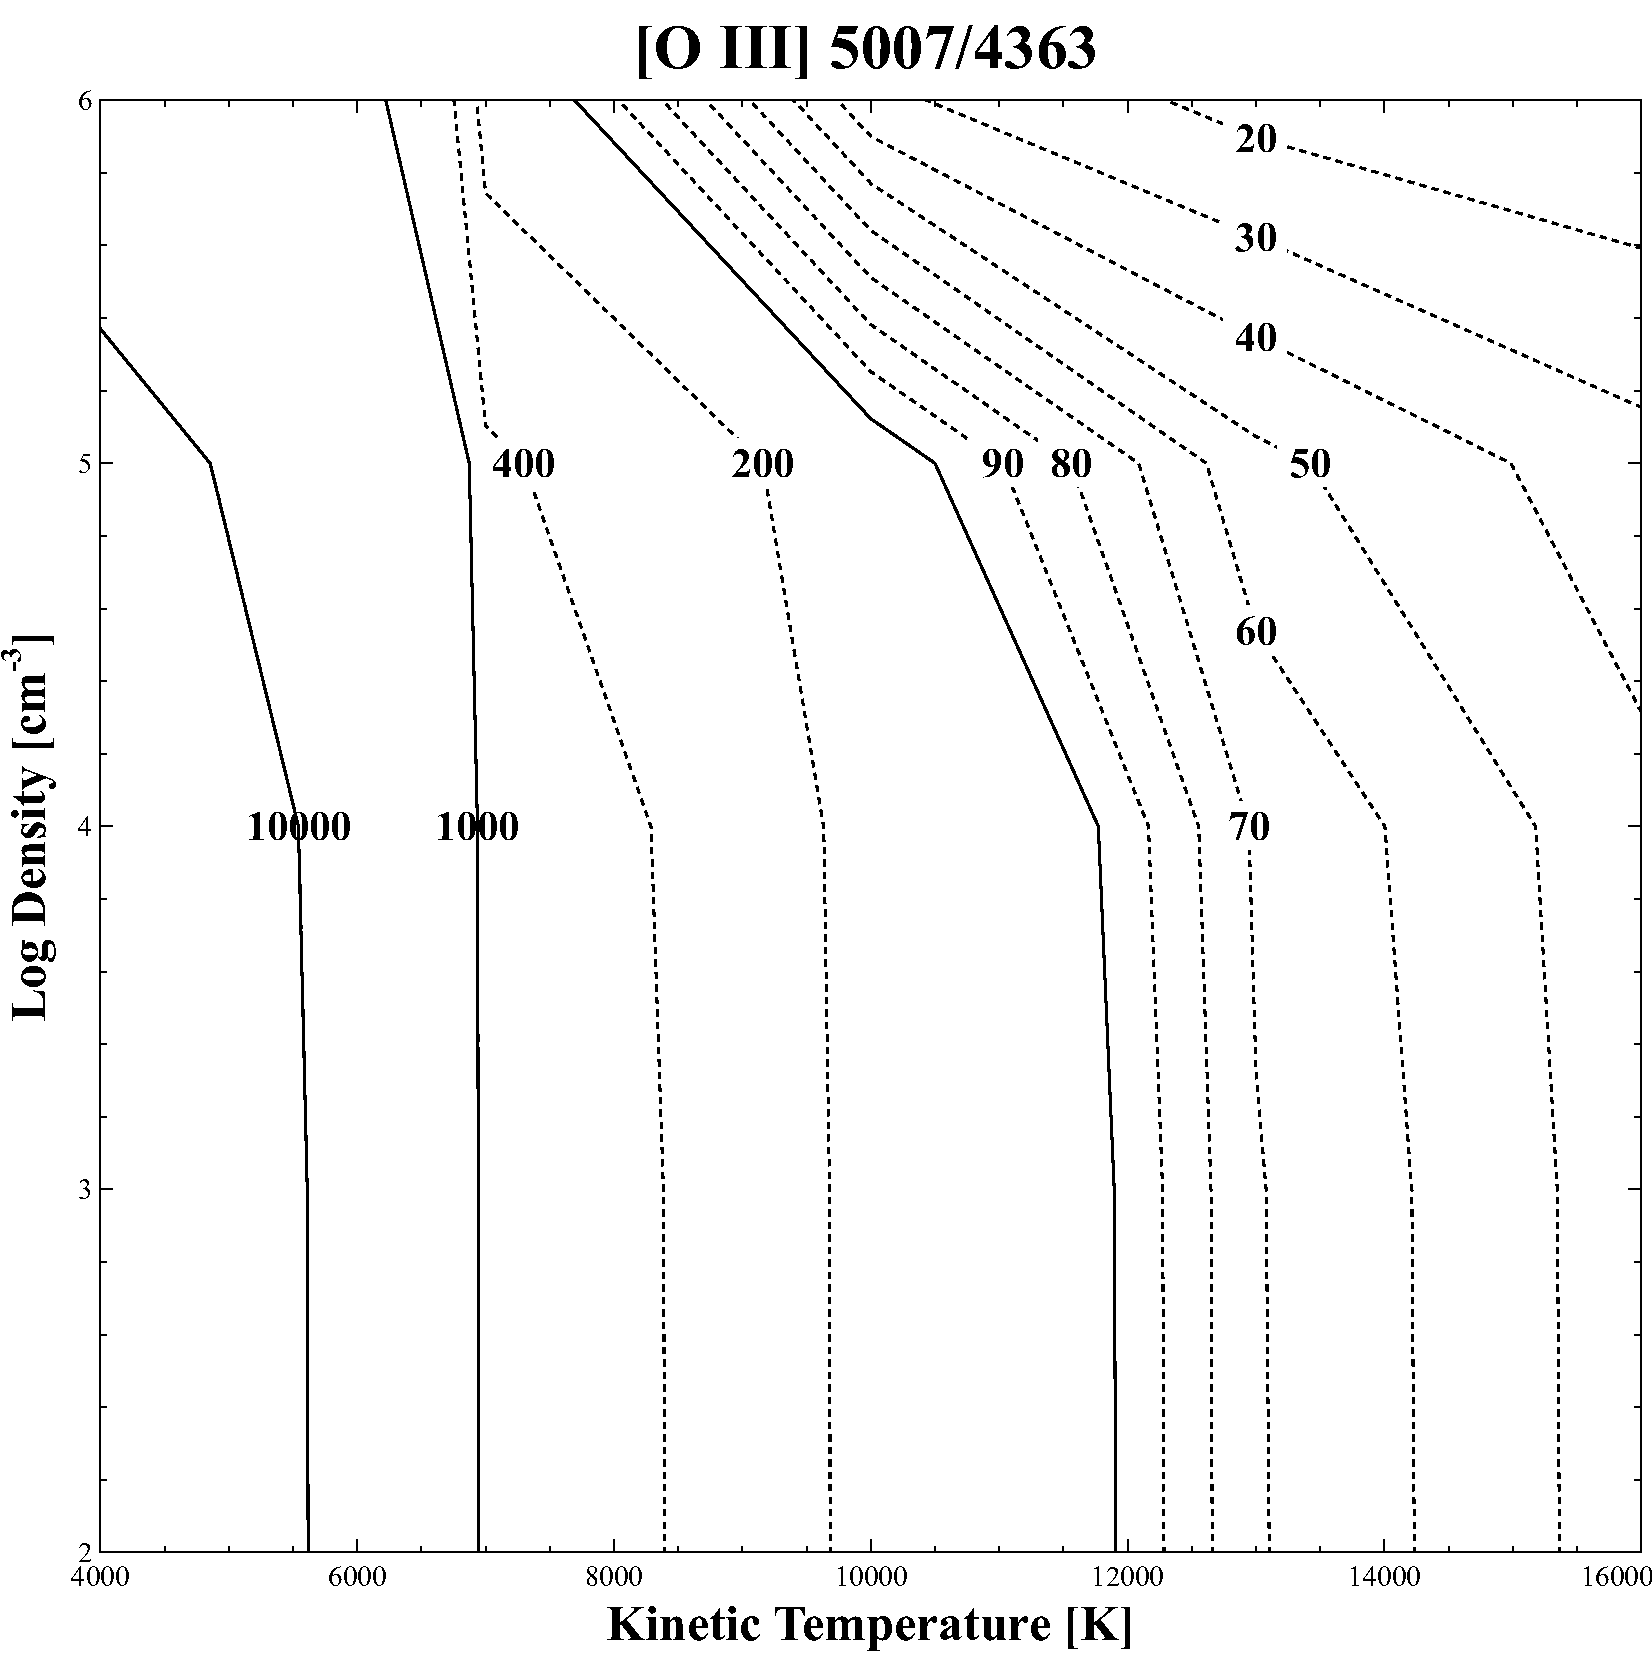
\includegraphics[scale=0.4]{SaveLineRatio}
\caption[Save line ratio example]{
\label{fig:SaveLineRatio}
The [O III] line ratio as a function of density and temperature.}
\end{figure}

\subsection{Save line optical depths, limit=-2}

This gives the mean optical depths for all lines.  By default all lines
with optical depths greater than 0.1 will be included.  The lower limit
can be reset with the optional number that appears on the line---it is the
log of the smallest optical depth to be printed (including line overlap).
This command recognizes the \cdCommand{units} option so the line
wavelengths can be in any of the wavelength or energy units
understood by this option.

The line identification, element and ion, starts the output line, in
the form used in the usual emission-line printout.
Next follows the line's wavelength or energy.
Next, the line's total (including line overlap), and
specific (ignoring line overlap) optical depths are printed.
Finally, the damping constant is printed.
The optical depth is integrated over the model,
but the damping constant is evaluated for the
conditions in the last zone.
Results are reported for the last computed zone unless the \cdCommand{every} option
appears.

In an open geometry (the default) the optical depths are integrated over the slab.
In the case where \cdCommand{sphere static} 
(see section \ref{sec:CommandSphere}) is given we integrate over 
the near and far side
of the sphere, but in the case of an expanding sphere 
(the default for the \cdCommand{sphere} command) it is assumed that the 
approaching and receding parts of the sphere are Doppler shifted so much 
that there is no overlap between the line profiles any more.


\subsection{Save line optical depth some}

This saves the mean optical depth of up to 100 emission lines as a
function of depth into the cloud.  These must be requested for single
line components: the optical depth for blends will be reported as 0.

For converged models, the total optical depth through the cloud is the same
regardless of how it is accumulated (inward or transmitted).
The direction of integration becomes significant only when
considering the optical depth as a function of depth through
the cloud.
The command integrates the optical depth from
the illuminated face up to the current depth into the cloud.

The emission lines are specified on the input lines that follow the
command and end with a line with the keyword \cdCommand{end} in columns 1--3.
The format for entering spectral lines is described in Section~\ref{sec:SpecifySpectralLines}.

The save output begins with emission-line labels and wavelengths.  The
remaining output gives the optical depth structure.  The first column is the
depth [cm] into the cloud.  The remaining columns give the optical depth for each line.  

The following illustrates its use;
\begin{verbatim}
save lines, optical some, "lines.opt"
o  3 5006.84A
o  1 6300.30A
end of lines
\end{verbatim}

\subsection{Save line pressure.}

This produces a list of the most important contributors to the line
radiation pressure for each zone.

%------------------------------------------------------------------------------
\subsection{Save line populations
        [row [lower$\vert$upper$\vert$ratio$\vert$tspin]]}
\label{sec:CommandSaveHyperfinePops}

This saves the upper and lower level populations of the requested spectral
lines.\footnote{
Until 2022, the command reported the level populations of (almost) all lines
known to the code.
This caused the output to be several MB even for a single zone model.
The current output was chosen as more user-friendly.
}
The command expects two filenames to be given, each enclosed in double quotes.
The first specifies the output file, while the second contains the spectral
lines to be tracked.
For example,
%
\begin{verbatim}
save line populations "output.txt" "linelist.dat"
\end{verbatim}
%
will read lines from \cdFilename{linelist.dat} and save the output in
\cdFilename{output.txt}.

By default, there is one line of output per spectral line per zone.
Each output line lists the depth, the transition line label,
the lower and upper level densities, the ratio $(n_u/g_u)/(n_l/g_l)$,
and the corresponding excitation temperature.
An example drawn from work on hyperfine lines in galaxy clusters is the
following:
%
\begin{verbatim}
#depth       emline         nl          nu          (nu/gu)/(nl/gl)  Tspin
5.00000e-01  Fe26 348.000m  9.3587e-11  9.0239e-15  3.2141e-05       3.9964e+00
5.00000e-01  Fe24 3068.00m  1.2614e-08  1.0044e-08  2.6540e-01       3.5353e+00
\end{verbatim}

If the \cdCommand{row} keyword appears, the command will generate one line of
output for each zone, listing the depth, and for each spectral line, one of the
columns above.
By default, the population ratio is reported, but the lower level, upper level
populations, or the spin temperature may be reported, instead; the relevant
keywords are \cdCommand{ratio}, \cdCommand{lower}, \cdCommand{upper}, and
\cdCommand{tspin}, respectively.
For example, using the \cdCommand{row} option with the previous command,
modifies the output to
%
\begin{verbatim}
#depth       Fe26 348.000m  Fe24 3068.00m
5.00000e-01  3.2141e-05     2.6540e-01
\end{verbatim}

These results may be used in post-processing.
For instance, the population ratio, $(n_u/g_u)/(n_l/g_l)$, may be used by
external programs to correct absorption coefficients for stimulated emission.

\subsection{Save line RT}

This produces a file containing information concerning line radiative
transfer. A series of lines that specify which emission lines to produce
follow the command. The format for entering spectral lines is discussed in
Section~\ref{sec:SpecifySpectralLines}. The line list ends with a line that
starts with \cdCommand{end}.

\section{Save map, zone 3 [range 3999 to 4500]}

This produces a map of the heating and cooling rates as a function of
temperature.  The details of the map are described in the description of
the \cdCommand{map} command.
The first number is the zone
for the map, zero if only a map of the first zone

The optional keyword \cdCommand{range} specifies the temperature range of the map.
If this option is specified then the zone number must come first and is
followed by the lower and upper temperature limits to the map.
Both
temperatures will be interpreted as logs if the first number is $\leq 10$.
The keyword \cdCommand{linear} will force that interpretation.  If the temperature range
is specified then there must be three numbers on the line---the stopping
zone number followed by the lower and upper limits to the temperature.

Normally 20 steps occur between the lowest and highest temperature in
the map.
The number of steps is reset with the \cdCommand{set nmaps} command.

\section{Save molecules}

The densities [cm$^{-3}$] of all molecules will be saved.  The depth and
the point and extended visual extinction into the cloud are given in the
first three columns.  The first line of the output gives header labels for
the molecules.

The \cdCommand{save species} command, section~\ref{sec:SaveSpecies},
allows the molecules to be printed to be chosen (or all molecules to
be printed, if the \cdCommand{all} option is used), so will generally
be more useful unless both the extinctions and {\em all}\/ molecules
are required.  The \cdCommand{save molecules} command will be removed
in a future release.

\section{Save opacities [total, grain, element]}

This gives some of the opacity sources considered by the code. The photon
energy is given in the first column and the opacities are in the columns that
follow. This command recognizes the \cdCommand{units} option to change the
energy scale. One of the keywords described in the following sections must
appear.

The opacities are only defined over the energy range over which the incident
radiation field is defined. The resulting opacities will not extend to high energies
for softer continua. A hard continuum such as \cdCommand{table agn} should use
used in the input stream to obtain the opacities over the full energy range.

Results are reported for the last computed zone unless the \cdCommand{every} option
appears.

\subsection{Save total opacity}

If the keyword \cdCommand{total} appears then the total opacity $\kappa$,
the absorption
cross section multiplied by the density of the absorber, summed over all
constituents, will be saved.
This has units cm$^{-1}$.
The optical depth would
be $\kappa $ multiplied by a physical depth.  This opacity includes all constituents,
gas phase and grains, for the last computed zone, with unit filling factor.
The first column is the photon energy and the second is the total opacity.
The absorption and scattering opacities follow.  The fifth column gives
the albedo, the ratio $\kappa _s /( {\kappa _s  + \kappa _\nu  }$).   The
$\kappa $'s are the scattering and absorption parts of the total continuous
opacity.  The last column is a label indicating the ionization edge for
each species included in the calculation.

\subsection{Save grain opacity}

The total grain cross section per hydrogen [cm$^2$/H],
for all grain types that are included, will be
saved after the last zone is calculated.  Successive columns give the
photon energy, the total (absorption plus scattering) cross section per hydrogen, 
the absorption cross section per hydrogen, and the scattering cross section per hydrogen.  The total and scattering opacity
discount forward scattering so are for the extended source case.  The last
column gives the scattering cross section per hydrogen with forward scattering included so
is for the stellar case.

\subsection{Save fine opacities range 0.7 to 1 Ryd, coadd 15 cells}

The code's execution time is partially set by the resolution of the
continuum mesh due to the need for frequent reevaluations of opacities and
rates.
A very fine continuum mesh, with resolution of 1~km~s$^{-1}$ or better,
is used to automatically treat line overlap.
The main opacity array cannot
use this resolution because single models would then have \emph{very} long execution
times.
Instead, the code uses a multi-grid approach where a coarse continuum
is used for most integrated quantities but a fine continuum grid is also
present to handle the line overlap problem.  This command will output the
current contents of the fine opacity array.  This only includes lines, not
continuous
emission or absorption from the cloud.

The resulting output file
will be huge.  Several options make the file smaller.
If the keyword \cdCommand{range} occurs then the first two numbers on
the command line are the lower and upper bounds to the energy range in the
output.  If neither is specified then the full energy range is reported.
The \cdCommand{units} keyword, described on \pageref{output_units},
can be used to change the units of both the range and the resulting output.

The last optional number says how many neighboring cells to co-add.  If
no number appears then 10 are coadded to reduce the amount of output.
This must be the third number on the line, so the \cdCommand{range} option
must also be specified to change the number of cells to coadd.

By default, only cells with non-zero opacity will be output.  
The keyword \cdCommand{ all} will report all cells.

\subsection{Save element opacity [name]}

If neither the \cdCommand{total} or \cdCommand{grains} keywords appear then the name of an element must be specified.
The keyword consists of the first four characters of
any one of the \LIMELM\ elements now incorporated in the code.
The photon energy
(eV) and total photoionization cross section (Megabarns [10$^{-18}
\mathrm{cm}^{-2}$]) for
all stages of ionization of the specified element will be saved.
A save
file name must still be specified to get past the command line parser but
is totally ignored.

The photoionization cross section of each stage of ionization is saved
in a series of files.  The name of the file will start with the first four
characters of the element's name, followed by the stage of ionization (the
atom is one), ending with \cdFilename{.opc}.  Examples are \cdFilename{CARB1.opc} or
\cdFilename{CARB6.opc}.

The code stops after producing these files.
Only one element can be treated at a time because of this.
If you want to examine the opacity files for more than one element
you will need to run the code one time with each element.

This version of the \cdCommand{save opacity} command is misnamed.
It actually saves the photoionization cross section, not the opacity due to the element.

\subsection{Save opacity figure}

This version of the command creates the file needed to generate one of
the figures used in another Part of \Hazy.
The output gives the energy in Rydbergs,
then keV, following by the hydrogen, helium, and total gas opacities.
The
opacities are in units of $10^{24} \mathrm{cm}^{-2}$ and have been multiplied by the cube
of the energy in Rydbergs.

\subsection{Save opacity shell 26 5 3}

This saves the state-specific photoionization cross section for a
subshell of any species.  The first number is the atomic number of the
element, the second number the ionization stage, 1 for an atom, and the
third number the subshell, between 1 and 7 representing $1s, 2s, 2p$, etc.
The save file will contain the incident photon energy in Rydbergs
followed by the cross section [cm$^2$].

\subsection{Save brems opacity}

This saves the free-free (a.k.a.\ brems) opacity of the gas as a function of
frequency in the last computed zone. The first column gives the frequency in
Rydberg, the second column the regular free-free opacity (between electrons
and ions), and the third column the electron-electron brems opacity. The
latter two quantities both have units cm$^{-1}$.

\section{Save optical depths}

This gives the total, absorption, and scattering continuum optical depths
for the computed geometry.  For a spherical geometry this is the optical
depth from the illuminated face to the outer edge of the cloud and not the
total optical depth.  The photon energy is followed by the total absorption
and scattering optical depths.
This command recognizes the \cdCommand{units} option
to change the energy scale.

\subsection{Save fine optical depths}

The code's execution time is partially set by the resolution of the
continuum mesh, due to frequent reevaluations of opacities and rates.
For problems related to line overlap, a very fine continuum mesh, with resolution
of 1~km~s$^{-1}$ or better, is used.
The main continuum array cannot use this
resolution because single models would then have \emph{very} long execution times.
Instead, the code uses a multi-scale approach, where a coarse continuum
is used for most integrated quantities, but a fine continuum grid is also
present to handle the line overlap problem.  This command gives the current
contents of the fine optical depth array.  This only includes lines, not
the continuum.

The resulting output file
will be huge.  Several options make the file smaller.
If the keyword \cdCommand{range} occurs then the first two numbers on
the command line are the lower and upper bounds to the energy range in the
output.  If neither is specified then the full energy range is reported.
The \cdCommand{units} keyword, described on \pageref{output_units},
can be used to change the units of both the range and the resulting output.

The last optional number says how many neighboring cells to co-add.  If
no number appears then 10 are coadded to reduce the amount of output.
This must be the third number on the line, so the \cdCommand{range} option
must also be specified to change the number of cells to coadd.

By default, only cells with non-zero opacity will be output.  
The keyword \cdCommand{ all} will report all cells.

\section{Save OTS}

The line and continuum on-the-spot fields will be saved.

\section{Save overview}

This saves an overview of the thermal and ionization structure
of the cloud and is a major output mechanism for the code.
The first numbers
are the depth [cm], temperature [K], local heating [erg cm$^{-3}$~s$^{-1}$], total
hydrogen density [cm$^{-3}$], and electron density [cm$^{-3}$].

These are followed by various ionization fractions.  
The \htwo\ molecular fraction is expressed as
$2n(\mathrm{H}_2)/n(\mathrm{H})$.
Neutral and ionized hydrogen fractions are followed by the ionization
fractions for the three stages of ionization of helium, the carbon molecular
fraction $n$(CO)/$n$(C), the first four stages of ionization of carbon, 
C$^0$ through C$^{3+}$, and
the first six stages of oxygen.  The last columns give the visual extinction
(for point and extended extinction) and the optical depth at 912\AA\ 
from the illuminated face to the current
position.

All reported quantities are the value itself.
This command accepts the \cdCommand{\_log} option 
(page \pageref{sec:SaveLogOption}) to report quantities in the
log style used in C13 and before. 

\section{Save PDR}

This gives some quantities relevant to a photodissociation region (PDR).
The first column gives the depth into the cloud [cm].  The second is the
total hydrogen column density [cm$^{-2}$].  The gas kinetic temperature follows.
These are followed by the ratios of densities of \hO, 2\htwo\ and 2\htwo* to total
hydrogen, C$^0$ and CO to total carbon, and water to total oxygen.  The next
number is the (dimensionless) intensity of the UV continuum relative to
the Habing background. The last columns give the total extinction in
magnitudes in the $V$ filter measured from the illuminated face
of the cloud for a point and extended source.

\section{Save performance}

The code will output the zone number, the time required to compute that
zone, the elapsed time since the start of the calculation, and
the number of times per zone that the most nested (ionization) solver was called.
This is intended as a mechanism to identify zones that require large amounts of
work to converge. 

\section{Save pointers}

This gives the element number, ion stage, and the shell number, for all
shells of the elements heavier than helium.
This is followed by the energy
of the lower and upper ranges of this shell and the photoionization cross
sections at these bounds.

\section{Save physical conditions}

The physical conditions as a function of depth will be saved.  The
depth into the cloud [cm] is followed by the temperature [K], hydrogen and
electron densities [cm$^{-3}$], heating [erg cm$^{-3}$~s$^{-1}$], the radiative acceleration
[cm~s$^{-2}$], and filling factor.

\section{Save pressure}

Various contributors to the total pressure in the gas equation of state
will be saved.  Pressures are given in dynes cm$^{-2}$.
Successive columns give the following:
\begin{description}
\item \emph{depth} is the depth [cm] from the illuminated face to the center of the
current zone.

\item \emph{Pcorrect} is the correct pressure at the current position.  This is the
sum of all contributors to the total pressure.  This may include, among
other terms, gas, radiation, turbulent, magnetic, and ram pressure.

\item \emph{Pcurrent} is the current pressure.  It will be equal to the correct total
pressure, the previous term in the output, if the pressure has been
converged.  The tolerance on the pressure convergence is controlled with
the \cdCommand{set pressure convergence} command.

\item  \emph{PIn+Pinteg} is the sum of the gas and radiation pressure due to the
incident continuum evaluated at the current position.  In a hydrostatic
model, such as the Orion model proposed by \citet{Baldwin1991}, this will
be the total pressure and will be equal to the sum of the gas pressure at
the illuminated face and the momentum absorbed from the incident continuum.

\item \emph{Pgas(r0)} is the gas pressure at the illuminated face of the cloud.

\item \emph{Pgas} is the current gas pressure.

\item \emph{Pram} is the current ram pressure.  This is only non-zero if the gas is
moving, which only occurs when the wind geometry is computed.

\item \emph{Prad(line)} is the current line radiation pressure.

\item \emph{Pinteg} is the current integrated pressure due to attenuation of the
incident continuum.

\item \emph{V(wind km/s)} is the wind velocity in km s$^{-1}$.  This is only non-zero for
a wind geometry.

\item  \emph{cad(wind km/s)} is adiabatic sound speed in km s$^{-1}$.

\item \emph{P(mag)} is magnetic pressure at the current position.

\item \emph{V(turb km/s)} is the turbulent velocity in km s$^{-1}$.

\item \emph{P(turb)} is the turbulent pressure.

\item \emph{int thin elec} the integrated radiation force
for electron scattering opacity only, in the absence of
any absorption.

\item  \emph{conv} This is ``T'' if the pressure is conserved and ``F'' if it is not.
\end{description}

\section{Save qheat}

The probability distribution for the grain temperatures is saved.
The first column is the grain temperature and the second column gives
$dP/d\ln T$ as defined using the nomenclature of \citet{Guhathakurta1989}.
Peter van Hoof added this command.

\section{Save radius}

The zone number is followed by the distance to the central object, the
depth to the illuminated face of the cloud, and the zone thickness, all
in cm.  If the keyword \cdCommand{outer} appears then it will only write this information
for the outer radius.

\section{Save recombination [option]}

\subsection{Save recombination coefficients}

Total recombination coefficients, the sum of radiative, dielectronic
and three-body, will be produced for all elements in the code.  These rate
coefficients [cm$^3 \mathrm{s}^{-1}$] are evaluated at the current electron temperature.

\subsection{Save recombination efficiency}

This gives the recombination efficiency for hydrogen, singlet helium
and the helium ion.

\section{Save results}

The intrinsic intensities of all emission lines with non-zero
intensities, and all column densities,
can be saved at the end of the calculation by entering the command \cdCommand{save results last iteration}.
This is one way to save the results of a grid of
models.
The resulting file contains the entire input stream as well.

The resulting save output will have the line information spread over
6 columns.
For some data base applications it would be better to have a
single column of results.
If the keyword \cdCommand{column} appears then a single column
is produced.
If no keyword occurs, or the keyword \cdCommand{array} does, then the
wide format is produced.

\section{Save secondaries}

The rate of secondary ionization of \hO, dissociation of \htwo,
and excitation
of \hi\ L$\alpha $, are given as a function of depth into the cloud.

\section{Save source function [depth, spectrum]}

\subsection{Save source function, spectrum}

The continuum source function for the local diffuse radiation field will
be saved.  The first column is the photon energy.  The second column is
the diffuse radiation field at that energy, in units of photons per second
per Rydberg.
Column three contains the total absorption opacity [cm$^{-1}$]
at that energy.
Column 4 contains the source function, the ratio of the
diffuse field to opacity (both have the units described above).
The last
column gives this ratio relative to the Planck function at the local
electron temperature.

The last column is a measure of the local source function relative to
the local Planck function.
This will generally be nearly unity for a thermal
plasma close to LTE.
Ground states of atoms of hydrogen and helium generally
have departure coefficients greater than unity so this ratio will be less
than unity at energies when their emission dominates.  The helium ion can
have departure coefficients much smaller than unity for nebular conditions
so the source function at helium-ionizing energies can be greater than the
Planck function.

\subsection{Save source function, depth}

The source function of the diffuse field at an energy slightly greater
than the Lyman continuum edge will be saved for all depths into the cloud.
All quantities are evaluated at the lowest energy continuum cell that lies
within the Lyman continuum.  The first column gives the integrated optical
depth from the illuminated face of the cloud to the current position.  The
second is the ratio of the diffuse field (photons per Rydberg per second)
to the absorption opacity.  The third is the OTS continuum at this frequency,
and the last is the ratio of the OTS continuum to the opacity, a photon
measure of the OTS source function.

%=============================================
\section{Save species [options]}
\label{sec:SaveSpecies}

These commands provide information about the molecules, atoms, and ions that are
treated by a unified ``species'' approach.
Options described below specify what information, for instance,
population or column density, to report.
If an ion or molecule is resolved into levels then the quantity for each
level is reported.
\textbf{Note that the reported levels are in the same order as in the input
atomic data models.}\footnote{\Cloudy{} sorts the levels internally, so the
calculations are correct and self-consistent.
We report results in the input order to keep them intelligible.
Users are advised to review the input database models when level-resolved output
is requested.}
For unresolved species only the total is given.
The rules for how different species are defined is given on 
page \pageref{sec:SpeciesDefine} above.

\textbf{\textit{Warning about ortho/para resolved LAMDA models}}
Several molecule models in the third-party database LAMDA separate species 
into ortho- and para- systems.  
The  \cdCommand{save species} command in this version of Cloudy has the limitation that 
only the last system in the LAMDA masterlist will be reported in the output.
This affects only the output of these commands.
All recognized systems will be included in the simulation.

The \cdCommand{save species} commands are of two types.
The first group reports derived physical quantities such as the column density
in various levels within the species.
The second group reports fundamental physical properties of the model,
such as the levels, line collision strengths, etc.

\subsection{Saving derived physical quantities}
\label{sec:SaveSpeciesDerived}

\subsubsection{Specifying a particular species}
By default this command 
reports details about a list of species, each
on a new line and without quotes, followed by \cdCommand{end}.

It is possible to specify only one species matcher by including its
label in double quotes, as well as a single-element list.  Some
rules:
\begin{itemize}
  \item The file name for the saved data must appear as the first
  item in double quotes.  Any species label comes second.
  \item The species label must match one of the labels 
  given with the \cdCommand{save species labels} command.
  These are case sensitive.
  \item The rules for how the species labels work are defined on 
  page \pageref{sec:SpeciesDefine} above.
\end{itemize}

The \cdCommand{all} option will print all molecules and ions which exist
in the calculation.

\subsubsection{Level populations}
\label{sec:SaveSpeciesLevelPopulations}

In addition, individual states of level-resolved species can be
accessed by including the level index in square brackets after the
species name, e.g.\@ \verb|"He+[1]"| or \verb|"CO[2]"|, or a range of
levels if range indexing is used e.g.\@ \verb|"He+[1:5]"|.  
The indices are on the physics scale so count from a lowest level of 1.
If the
lower bound is omitted, the range starts at the lowest available
level, likewise if the upper bound is omitted, so \verb|"He+[:]"|
prints all levels.  The individual levels are not reported by the
\cdCommand{save species labels} command.
  
The total for the species will be reported if the species name is specified
without the square brackets, as in \verb|"CO"|.  The population of the
lowest level will be reported if  \verb|"CO[1]"| is specified.

\subsubsection{Other quantities}
\begin{table}
\caption{Other quantities which can be added as columns in \protect\cdCommand{save species}.}
\begin{center}
\begin{tabular}{ll}
\verb|*depth| & zone depth \\
\verb|*AV| & point AV \\
\verb|*AVx| & extended AV \\
\verb|*temp| & temperature \\
\verb|*time| & elapsed time (for time-dependent calculations)
\end{tabular}
\end{center}
\label{tab:othersaves}
\end{table}
Other quantities can also be printed, as shown in Table~\ref{tab:othersaves}.

\subsubsection{Examples}

The following gives examples:
\begin{verbatim}
#
# save total water column density
save species column density "pdr.col" "H2O"
#
# ions use baryon, not spectroscopic, notation.  This is C IV == C+3
save species populations "flow.pop"  "C+3"
#
# save set of species, some for particular levels
# total in C+, populations in the first two levels of C+, the lowest level of CO,
# the electron density and the point visual extinction
save species densities "pdr.pop"
"C+"
"C+[1:2]"
"CO[1]"
"e-"
"*AV"
end
\end{verbatim}

\subsubsection{Save species column densities}
This reports the column densities [\pscm] at the end of the iteration.

\subsubsection{Save species departure coefficients}
This reports the departure coefficients [dimensionless] for all zones.
The depth is given first, and then the departure coefficient for each
species.

\begin{verbatim}
# save all levels
save species departure coefficients "sim.dep" "H[:]" 
# only save total for atom
save species departure coefficients "sim.dep" "H" 
\end{verbatim}

\subsubsection{Save species densities}
This reports the density of species and of levels [\pccm] for all zones.
The depth is given first, and then the density for each species.

\subsubsection{Save species optical depths}
This saves the optical depths of all lines.
The lower and upper index of the transition is followed by
the line optical depth.
We report line-center optical depths.

\subsubsection{Save species levels}
This reports the number of levels used for each species, for each zone.
If a species is not resolved, that is, it has no internal structure,
the number of levels will be given as zero.
This provides a way to watch the number of levels in a model change
as the physical conditions change.

Tables giving the energy levels, their designation, and statistical weight,
are contained in ``energy'' files located within each database.

\subsubsection{Save species continuum [units Ryd] [row [inward, outward]]}
\label{sec:SaveSpeciesContinuum}
This reports the pseudo-continuum of a species, that is, its (line)
emission in a given wavelength range.
The output file name, and the species must be specified in that
order in double quotations, as in
%
\begin{verbatim}
save species continuum "feii.pseudo-cont" "Fe+"
\end{verbatim}
%
By default, the continuum band is from \speciesConWlLo{} to \speciesConWlHi{}, 
split in \speciesConNbins{} logarithmic bins.
These defaults can be modified with the \cdCommand{set species continuum}
command, described in Section~\ref{sec:SetSpeciesContinuum}.

\par
The output file lists the photon energy, the total intensity,
and the intensity directed inward, and outward, in that order,
in four tab-delimited columns.
The photon energy is reported in Ryd, unless other units are
specified with the \cdCommand{units} option.
The units of the intensity in the intensity and luminosity
cases follow those for the \cdCommand{save continuum} command,
described in Section~\ref{sec:CommandSaveContinuum}.

Because for large grids of calculations, this format may prove
inconvenient, the \cdCommand{row} option is provided.
When issued, the wavelengths are listed once, in a single row
at the top of the file, with subsequent rows holding the intensities
for various grid points.
Only one intensity sum is then reported per grid point,
by default the total intensity.
This may be altered by issuing the \cdCommand{inward} or
\cdCommand{outward} options, which will cause the corresponding
intensity to be reported instead.

The distinction between total, inward- and outward-directed emission
is important, e.g., for Fe~{\sc ii} lines in quasars, as discussed
by \citet{FerlandHuEtAl2009}.


\subsubsection{Save species bands}
\label{sec:SaveSpeciesBands}

\par
This command accepts a file that contains a number of bands over which the
line emission of the indicated species is computed. The results are stored
in the specified output file, and are also reported in the emission line
list in the main output.

\par
For example, the following computes the emission of the ``Fe+'' species
over the bands found in \cdFilename{data/FeII\_bands.ini},
%
\begin{verbatim}
save species bands "bands.feii" "FeII_bands.ini" "Fe+"
\end{verbatim}
%
The first file to appear in the command is the output file,
the second is the bands file, followed by the species of choice.

\par
A user-defined bands file may be used instead, but it must follow the
format of file \cdFilename{data/FeII\_bands.ini}.
Briefly, each line holds one band only, described by three (positive)
wavelengths, all in Angstr\"{o}m.
The first column holds the wavelength that will be used with reporting,
and the following two columns hold the minimum and maximum wavelengths
of the band, in that order.
The remainder of the line is ignored.
Comment lines, which begin with a hash (\#), are ignored.
Bands are independent of each other, which means that they are not
expected in any specific order, and they may also overlap.

\par
The output created in the file specified by the \cdCommand{save} command
has four tab-delimited columns.
The first column reports the wavelength of the band specified in the
first column of the (input) bands file.
The following three columns report the total, inward, and outward
species line emission over that band.
The intensity units follow those for the \cdCommand{save continuum} command,
Section~\ref{sec:CommandSaveContinuum}.
By default, intrinsic intensities are reported; for emergent intensities the
keyword \cdCommand{emergent} may be used.

\par
The bands will appear in the main output only if a \cdCommand{save} command is
entered.
The only exception to this rule is the ``FeII'' bands file: it is always parsed,
and the summed up emission always appears in the main output.

\par
There, the bands are identified by the spectral label of the species, followed
by a single `b'; e.g., the band for ``Fe+'' is ``Fe 2b''.
This is then followed by the wavelength of the band, listed in the
first column of the bands file.
This entry contains the sum of the inward and outward flux. For each of the
bands a second entry will be created that only contains the inward flux.
These entries will have the label ``InwdBnd'' followed by the wavelength of
the band.
See also Hazy 2, Section~\ref{Hazy2-sec:SpeciesBands}.

\subsection{Save species optical depths}
\label{sec:SaveSpeciesOpticalDepths}
This reports the optical depths of all lines for the specified species.
The first two columns give the index of the upper and lower levels, in
that order, on the physics (not C) scale, the third column gives the
wavelength of the transition in Angstrom, and the last column gives
the mean optical depth.


\subsection{Saving fundamental physical properties of the species}

\subsubsection{Save species energies}
This reports the level energies.  The default is to give level
energies in Rydbergs but this can be changed with the
\cdCommand{units} keyword.  The energies are reported relative to the
ground state of the species.  This command is useful for identifying
excitation levels from their index numbers, and should generally be
given a range of levels as its argument, e.g.
\begin{verbatim}
save species energies "test_h_all.nrg" "H[:]"
save species energies "test_h_some.nrg" "H[:10]"
\end{verbatim}
The energies for molecular species are reported as zero.

\subsubsection{Save species labels}
\label{sec:SaveSpeciesLabels}
This gives a list of the species labels, a useful way to find out how
we refer to a particular atom, ion or molecule.  This command will
typically be used with the \cdCommand{all} option, to give an
inclusive list.
Each entry also lists the external database from which the atomic
data are derived, or the iso-sequence the species belongs to, if
appropriate.
If no database name exists then the species does not have internal structure.

\subsubsection{Save species lines [options]}
\label{sec:CommandSaveSpeciesLines}

This saves the atomic data that \Cloudy\ uses in a given simulation.
If the keyword \cdCommand{all} appears then data for
all active species are reported.
Otherwise, a species is expected, e.g., ``Si+5''.
Multiple instances of the command may be issued, but each species is
processed once across all files.
That is, if a species is requested for two output files, it will appear
only in the first file.

\par
By default for each transition the spectral label is reported,
followed by its wavelength, its lower/upper level indices,
the statistical weights of these levels, the Einstein A,
the collision strength, and a column that holds a flag,
in that order.
The flag indicates whether the g-bar approximation was used in
the calculation of the collision strength.
Values of -1 are appropriate for transitions from iso-sequence species.
All other species have values of 0 for transitions with collisional
data, and 1 for transitions without collisional data, for which the
g-bar approximation has been used.

\par
Optional keywords change this behavior.
The transition energy in wavenumbers is reported instead of the wavelength,
if the keyword \cdCommand{\_wn\_} appears. 
The oscillator strength is reported instead of the Einstein A,
if the keyword \cdCommand{\_gf\_} appears.
In addition, downward deexcitation rates for all possible colliders are reported,
if the keyword \cdCommand{rates} appears.
These rates are reported at the end of each line, after the g-bar column.


\subsubsection{Save species data sources}

This saves a table giving the data sources for atomic and molecular species that are
treated with external databases.  

%=============================================
\section{Save special}

If \cdCommand{special} is specified then routine
\cdRoutine{SaveSpecial} will be called.
This routine can be changed to fit the circumstances.

\section{Save tegrid}

The history of the last \cdVariable{NGRID} evaluations of the
heating and cooling will be saved.
\cdVariable{NGRID} is set in a header file.
This is one way to evaluate
the stability of the thermal solutions.

\section{Save temperature}

The radius is followed by the temperature and the derivative of the
cooling with respect to temperature $dC/dT$.
Next come the first and second spatial derivatives of the temperature
with respect to depth, $dT/dr$ and $d^2T/dr^2$.
These derivatives set the rates
of conductive heat flow and heat loss respectively.

\section{Save time dependent}
\label{sec:SaveTimeDependent}

This gives some information on a time-dependent model.

\section{Save TPredictor}

The code estimates the temperature of the next zone from the changes
in temperature that have occurred in previous zones.
This is only attempted
in a constant density geometry.
This output gives the old temperature,
the estimated new temperature, and the final equilibrium temperature.

\section{Save XSPEC atable \textbar\ mtable [ range 0.1 200 ] [~normalize [ 2.3 ] ]}

This command produces a file in FITS format for input into the spectral
analysis program XSPEC (\citealp{Arnaud1996}).
This command was added by Ryan Porter
and its first application is given in \citet{Porter2006}.

Either \cdCommand{atable} or \cdCommand{mtable} must be specified. These
keywords refer to additive and multiplicative tables respectively. This
command is used with the \cdCommand{grid} command to produce grids of
calculations. The file produced by this command contains predictions
pertaining to the last iteration of each of the simulations (i.e.\ the keyword
\cdCommand{last} is implicitly in effect). A file produced with
\cdCommand{mtable} contains the energy bins and total optical depth,
exp($-\tau$), from the illuminated face to the last zone of each simulation in
the grid including line absorption, but excluding any scattering processes.
A file produced with \cdCommand{atable} contains the energy bins and
some component of the spectrum, as determined by the following options:

\begin{description}
\item[total -] saves the sum of the outward spectrum and the reflected spectrum,
including diffuse and incident, lines and continua.

\item[{[ attenuated \textbar\ reflected ]} incident continuum -] saves the incident
continuum, the attenuated incident continuum or the reflected incident
continuum;

\item[{[ reflected ]} diffuse continuum -] saves the outward diffuse continuum
or the reflected diffuse continuum;

\item[{[ reflected ]} lines -] saves outward lines or reflected lines; and

\item[{[ reflected ]} spectrum -] saves the total outward spectrum or the total
reflected spectrum.
\end{description}

If none of these options are present, the total outward spectrum will be saved.
By ``reflected'' we mean components escaping into
the $2\pi$~sr subtended by the illuminated face toward the continuum source.
If no options are specified for the \cdCommand{atable} command then the transmitted
spectra will be saved.  Note that the command can be specified multiple
times, allowing the user to individually save any or all of the separate
components of the predicted spectra.

By default the full frequency range will be saved.  The \cdCommand{range} option
will limit the range.  Both lower and upper limits must be specified.  The energies
must be in keV.

By default the SEDs stored in an \cdCommand{atable} will be equal to the
equivalent SEDs from the \cdCommand{save continuum} command, except that they
have different units [photons\,cm$^{-2}$\,s$^{-1}$\,bin$^{-1}$] and
normalization will be forced on the inner radius (this is to prevent numerical
overflow). The saved spectrum will always conserve energy, i.e. the
\cdCommand{set save resolving power} command has no effect. There is an
optional keyword \cdCommand{normalize} that will cause the SED to be
normalized to 1 [photons\,cm$^{-2}$\,s$^{-1}$\,keV$^{-1}$] at a specific frequency. You can specify a number in keV to
set the normalization frequency, or it will default to 1 keV if that number is
omitted. If both the \cdCommand{range} and \cdCommand{normalize} keywords are
used, \cdCommand{range} (with its associated numbers) must come first. By
default the isotropic continua will be included. They can be excluded using
the \cdCommand{no isotropic continua report} command.

In the example below we specify that a blackbody is to be varied.
The
number on the \cdCommand{blackbody} line is ignored.
The \cdCommand{range} command specifies that
the log of the temperature of the blackbody will range from 4 to 6.
The
\cdCommand{grid} command specifies that we are calculating
a regularly spaced grid with 1 dex steps between 4 and 6.
In this case
since we only have one parameter varied with the \cdCommand{vary} keyword, there will
only be one dimension in the grid and only three simulations.
Each of the
two \cdCommand{save xspec atable} commands produces a FITS format file.  The first
file, named \cdFilename{filename1}, will contain the incident continuum for each of the
three simulations.
The second file, named \cdFilename{filename2}, will contain the
transmitted spectrum for each of the three simulations.
The commands are as follows:
\begin{verbatim}
blackbody 1e5 K vary
grid range 4 to 6 in 1 dex steps
save xspec atable incident continuum "filename1"
save xspec atable spectrum "filename2"
\end{verbatim}

\section{Save wind}

The radius and depth [cm] are followed by the velocity [cm s$^{-1}$],
total radiative acceleration [cm~s$^{-2}$],
the accelerations due to lines and continua
alone, and the dimensionless force multiplier.
If the keyword
\cdCommand{terminal}
appears then this is only produced for the last zone, otherwise it is for
every zone.
This option can be combined with the \cdCommand{save grid} command
to save predictions from a series of grid calculations.

\section{Title ``This is a title''}

The argument is a title for the calculation and can be useful for
organizing the models.  The preferred form is a quoted string, but if
this is not present, the whole of the line after the command will be
used for backward compatibility.

The title is reprinted several times to label output.

\section{Trace zone 94 [iteration 2; options . .]}

This command turns on \cdTerm{trace} information to follow
the logical flow within \Cloudy.
The code uses adaptive logic to control the calculation
and this option provides a way to follow these internal decisions.

The trace begins \emph{after} the zone given by the first number on the line.
If the zone is zero, or if no numbers occur on the line, then the trace
is turned on at the beginning of the calculation.  The second (optional
with default of 1) number is the iteration on which the trace should be
started.  It should be set to 2 to turn on the trace for the second
iteration.
So the command \cdCommand{trace 0 2} would start the trace at the
beginning of the second iteration.

Table \ref{tab:trace_conv} lists the trace keywords in the first column.
The four-character part
of the key that must be matched is capitalized.
The purpose of each is indicated in the last column.

A string including the word \cdMono{DEBUG} is printed when the
\cdCommand{trace} command is parsed.
This will not be printed if the option \cdCommand{no print} occurs
on the \cdCommand{trace} command.

\begin{table}
\centering
\caption{\label{tab:trace_conv}Trace convergence keywords and routines}
\begin{tabular}{ll}
\hline
Keyword& Routine\\
\hline
\cdCommand{pressure}& ConvPresTempEdenIoniz\\
\cdCommand{temperature}& ConvTempEdenIoniz\\
\cdCommand{eden}& ConvEdenIoniz\\
\cdCommand{ionization}& ConvIoniz\\
\hline
\end{tabular}
\end{table}

\subsection{Trace convergence level}

This is a special form of the \cdCommand{trace} command that prints an overview of
the decisions made during the calculation.
The physical state of the gas
is determined by nested pressure, temperature, electron density, and
ionization solvers.
This \cdCommand{trace} option makes it possible to view the
decisions made by any of these solvers.

The code will check for one of the keywords
\cdCommand{pressure}, \cdCommand{temperature}, \cdCommand{eden},
or \cdCommand{ionization},
and produce output explaining the decisions made by that
solver and all higher ones.
With no keyword all levels are printed.
Successively deeper layers are obtained with the keywords listed in
Table \ref{tab:trace_conv}.

There are further keywords that create additional printout.
The \cdCommand{OTS}
keyword will identify source of OTS fields.
The \cdCommand{ESOURCE} option will identify
sources of free electrons.

\subsection{Trace H-like [element name, full]}

This turns on extensive printout describing the physics of one of the
model hydrogenic atoms. The same code is used to compute atomic properties
for all hydrogenic species.  If the keyword \cdCommand{full} appears then the printout
will be far more detailed.  If no element is specified then this will only
be for hydrogen itself.  If the name of any other element appears then the
printout will be for that element.

\subsection{Trace He-like [element name, full]}

This turns on extensive printout describing the physics of one of the
model helium-like sequence atoms.  The same code is used for all helium-like
species.
If the keyword \cdCommand{full} appears then the printout will be far more
detailed.
If no element is specified then this will only be for helium
itself.
If the name of any other element appears then the printout will
describe that element.

\begin{table}
\centering
\caption{\label{tab:trace_keywords}Trace Keywords and Effects}
\begin{tabular}{ll}
\hline
Keyword& Quantity traced\\
\hline
BETA& OI 8446-\la\ problem\\
CARBon& carbon ionization
equilibrium\\
CALCium& calcium ionization balance\\
COMPton& Compton heating,
cooling,  and ionization\\
CONTinuum& prints out photon arrays,
pointers\\
CONVergence& convergence loop, no other
printout\\
COOLants& cooling\\
DIFFuse fields& sum of recombination coef in
DIFFEM\\
DR& choice of next zone thickness\\
EDEN& changes in electron
density\\
GRAIN& details dealing with grain
treatment\\
HEATing& heating agents\\
HEAVies& heavy element balance\\
HELIum& helium
ionization equilibrium\\
HELIum ATOM& Helium singlets ionization
equilibrium\\
HELIum IONized& helium ion ionization equilibrium\\
HELIum
SINGlet& Helium singlets ionization equilibrium\\
HELIum TRIPlet& helium ion
ionization equilibrium\\
HYDRogen& Minimal trce of the H ionization\\
IRON& Fe
abundance, K-alpha emission\\
LINEes& line pointers, opacity. A's,
etc\\
leveln& LevelN n level atom routine\\
Ly BETA& L$\beta$ - OI 8446 pumping
problem\\
MOLEcules& rate
coefficients for molecules\\
NEON& recombination, ionization for neon\\
OPTICal
depths& inner, outer optical depths in STARTR\\
OPTIMizer& Steps in optimize
command driver\\
OTS& ots ionization rates\\
POINters& pointers for element
thresholds\\
THREe body& three-body recombination rates for metals\\
TWO
photon& induced two photon processes\\
WIND& Wind geometry\\
\hline
\end{tabular}
\end{table}

